%----------------------------------------------------------------------------------------
\chapter{Design} 
\label{chap:design}
%----------------------------------------------------------------------------------------

In the previous chapters, it has been presented the necessary knowledge about the background research (\cref{chap:background}) and the platforms utilized in this work (\cref{chap:platforms}). 
This chapter discusses the conducted research from the design perspective, giving the main points and emphasizing the key ideas without going into the implementation details as the next chapter (\cref{chap:implementation}). 

As analyzed in the Intro (\cref{chap:introduction}), humans have remarkable cognitive flexibility and use it to achieve complex goals across various daily scenarios. These goals are often broken down into smaller sub-tasks (skills), and this is one objective of this research. This combination of trajectories also requires an appropriate shift among them, in both cases, the combination being end-to-end or partial. 

Being biologically inspired, this research aims to emulate this human flexibility in skill execution and task composition with the previously explained CNMP networks. Movement primitives that define skills are combined differently for different goals and are adapted to the environment and context thanks to the interpolation abilities of CNMP networks.

The following discussion will proceed with analyzing before the partial skill composition with CNMPs, modeling how it is possible to go from one movement primitive to the other. The motivation of this order is that this part enables the partial combination and is used as well in the transition moment of end-to-end skill concatenation.

Next, it will be analyzed how it is possible to concatenate them one after the other to achieve meaningful execution in order to reach the final goal position or even goal-state.

\newpage
%%%%%%%%%%%%%%%%%%%%%%%%%%%%%%%%%%%%%%%%%%%%%%%%
\section{Partial Skill Combination}
%%%%%%%%%%%%%%%%%%%%%%%%%%%%%%%%%%%%%%%%%%%%%%%%

% requires change action (shift TP) halfway
In order to synthesize a new skill by combining parts of others, it is required to teach the model at least two different types of movement primitives. Subsequently, the robot has to be able to pass from one action (skill) to the other. 

The moment of this transition has to be arbitrarily decided according to the necessities and not specifically crafted at teaching time. 

The challenge of this apparently straightforward problem resides in the moment of the transition, because it has to be executed in a meaningful, natural, and safe way. These simple three requirements will lead the following examination through different approaches till the one designed. 

For the purpose of a better understanding of the design and its steps, from now on, a simplistic example (\cref{fig:trajX}) will be used to further clarify the explanations given. Nevertheless, the simplification doesn't exclude the possibility of more elaborate tasks that require complex movements or sensorimotor data. 

The two actions discussed will be a simple movement upwards and a similar movement downwards. They can represent, for example, a trajectory in real life, a manipulator movement, or a joint trajectory. This allows a discussion that starts from a single 1D dimension and keeps the understanding manageable at the subsequent introduction of new dimensions. 

\begin{figure}
    \centering
    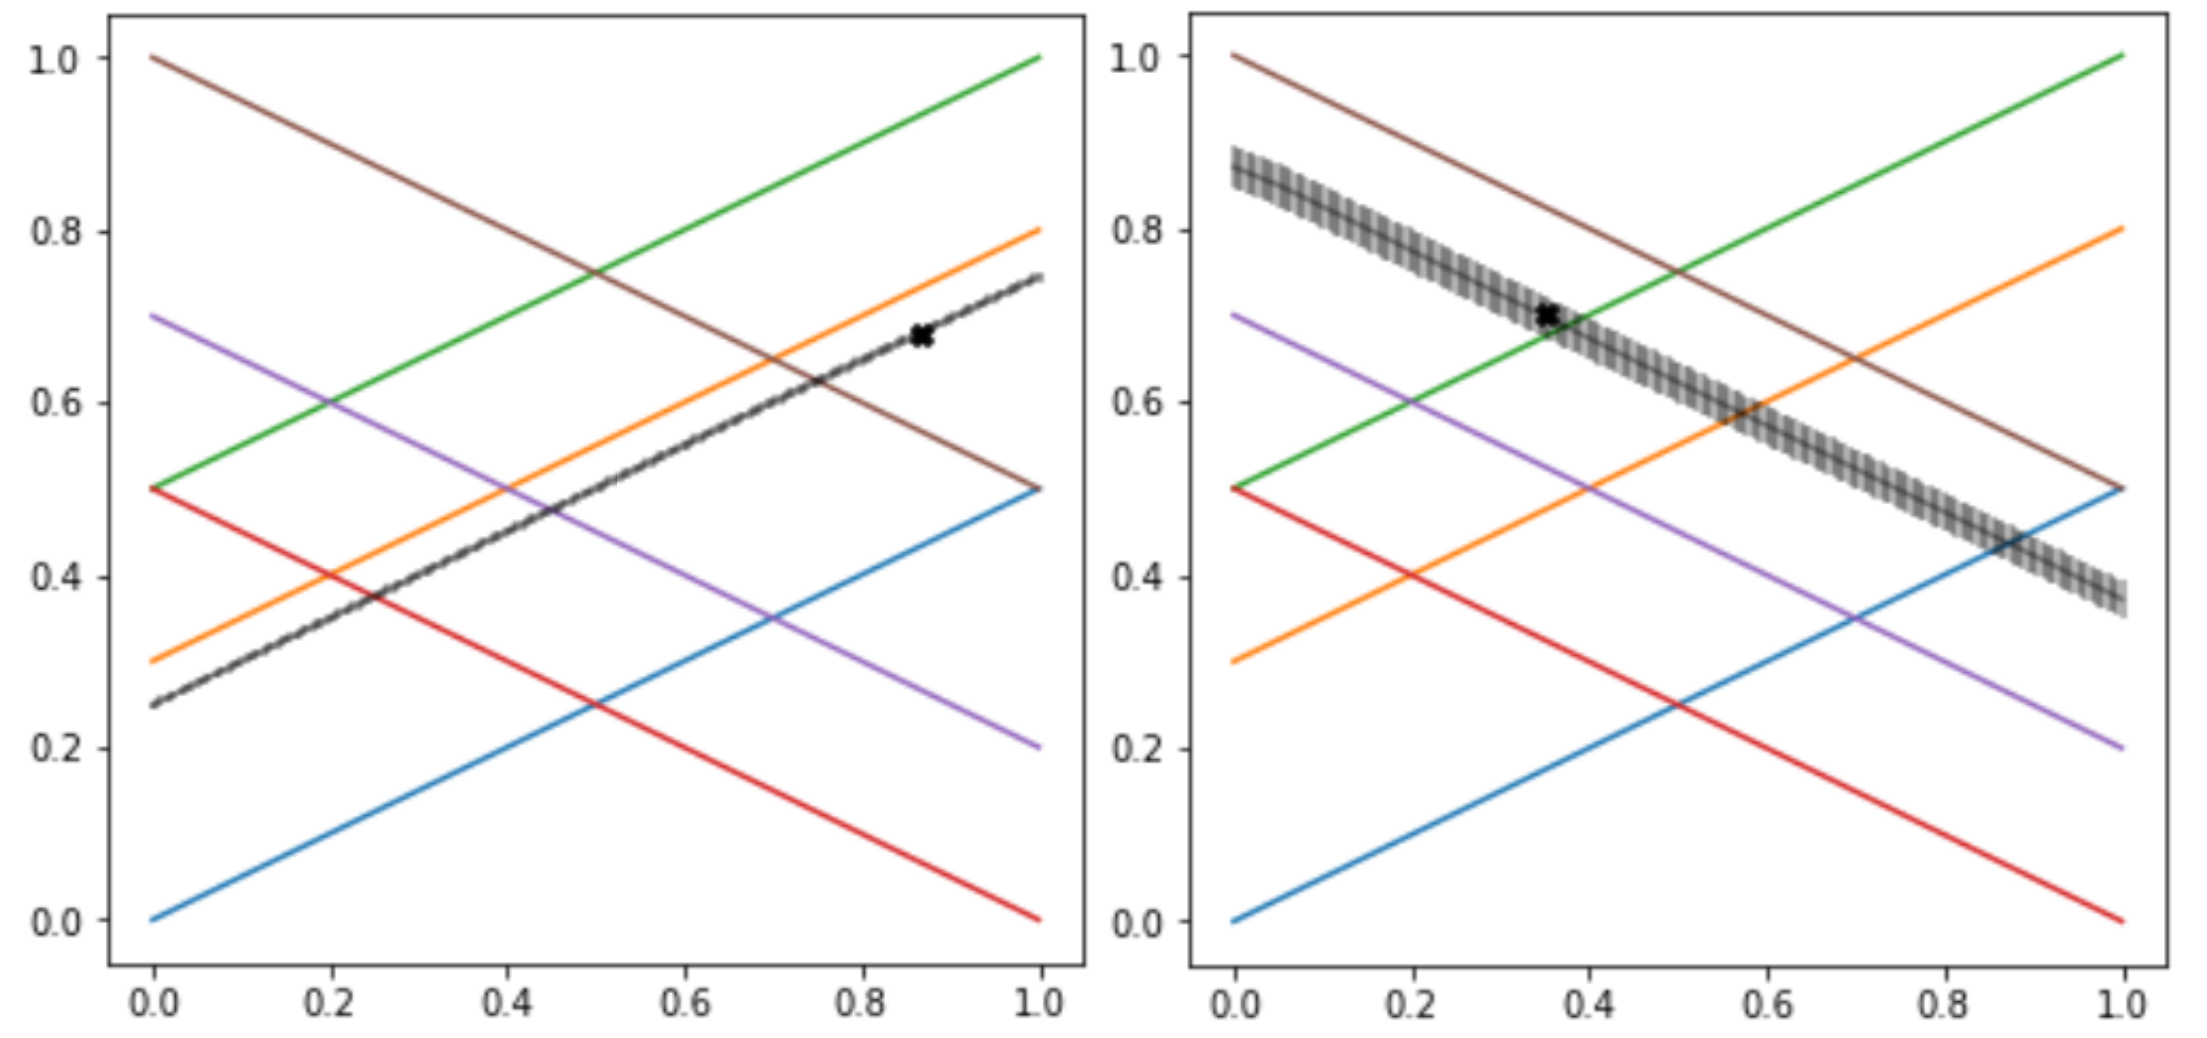
\includegraphics[width=0.8\linewidth]{figures/trajX.png}
    \caption{ Trajectories for two different skills demonstrated, in different colors. The generated ones in grey color, from the black conditioning points. }
    \label{fig:trajX}
\end{figure}

Some demonstration trajectories are given for both skills, in the \cref{fig:trajX} are visible as the three colorful thinner lines ascending and three colorful thinner lines descending. The two triplets differ to some extent, so the network has enough knowledge to create as well new trajectories never seen. This will prove later that the method designed also works with newly generated movement primitives. 

The thicker points in the \cref{fig:trajX} are the conditions, these force the model to generate a trajectory that passes through that state. The movement primitive created is denoted as the grey line passing through the condition point, along with the uncertainty of the prediction in every timestep as its width. 

% do it without jumps
The shift can not be abrupt, so it's not sufficient to directly stitch together two parts of the trajectories collected. 
The simplest solution of executing one trajectory till a certain desired timestep and executing the second one after that moment will create an abrupt jump in the execution for the majority of timesteps where the trajectories don't perfectly intersect (\cref{fig:trajX-failing-approaches}). A jump in the movement primitive will lead to an unnatural fast change of pace and position of the robot during the execution, which is not clearly referable to human behavior. Moreover, moving from one position to a completely different one in the next moment is an unsafe behavior. It might lead to damage to the robot itself and its surroundings, harm to people, or activate the safety stop measures of the robot due to the high speed and torque applied.  

\begin{figure}
    \centering
    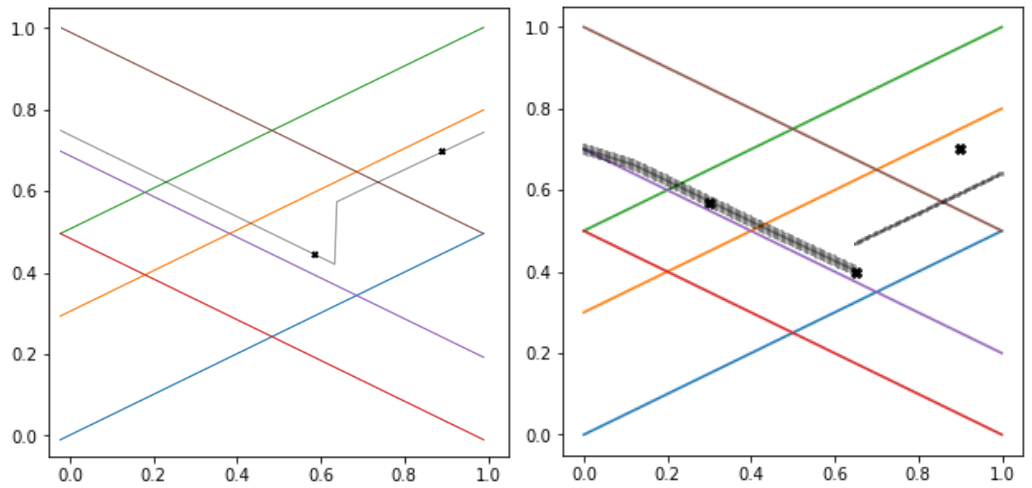
\includegraphics[width=0.8\linewidth]{figures/trajX-failing-approaches.png}
    \caption{Examples of failing approaches with stitching in CNMPs. On the left, simple combination of parts. On the right, stitching the right part using a conditioning point at the end of the left part.}
    \label{fig:trajX-failing-approaches}
\end{figure}

Being able through the CNMP model to generate trajectories from previous demonstrations allows a certain flexibility, so a second approach might suggest generating a second trajectory starting from the end points of the first one. This solution only delays the problem subsequently because the condition point(s) on the second trajectory will be dependent on the first one, requiring further calculation, and won't be solely used for the effective purpose of making a trajectory reach the desired state. In \cref{fig:trajX-failing-approaches}, right plot, the first part of the trajectory is generated with the left-most condition ($time=0.3$). Subsequently, the second part is generated using a conditioning point at the end of the left part plus the desired one. These two conditioning points will likely not be on the same trajectory generated: let's recall the robot arms generally have 6 or 7 DoF, \cref{chap:platforms}, and even the cartesian space has three dimensions plus the 4D quaternion for the orientation, so the probability of trajectories intersecting in spaces of at least six dimensions is minimal. This will lead the CNMP model to average the two trajectories obtained by the two conditions on different points. In \cref{fig:trajX-failing-approaches}, right plot, we see the second trajectory part passing in the middle of the two right-most observations that would generate independently two different movement primitives. To pass from one to another of these last two trajectories, a shift will still be required, and this raises again the same problem. 
So, even using conditioning points, there is a tradeoff between jumping and not meeting the conditions for the second trajectory.

% same network
Since the stitching of parts is not a feasible option, the approach selected implies giving the same network the two skills and obtaining a coherent output.

\begin{figure}
    \centering
    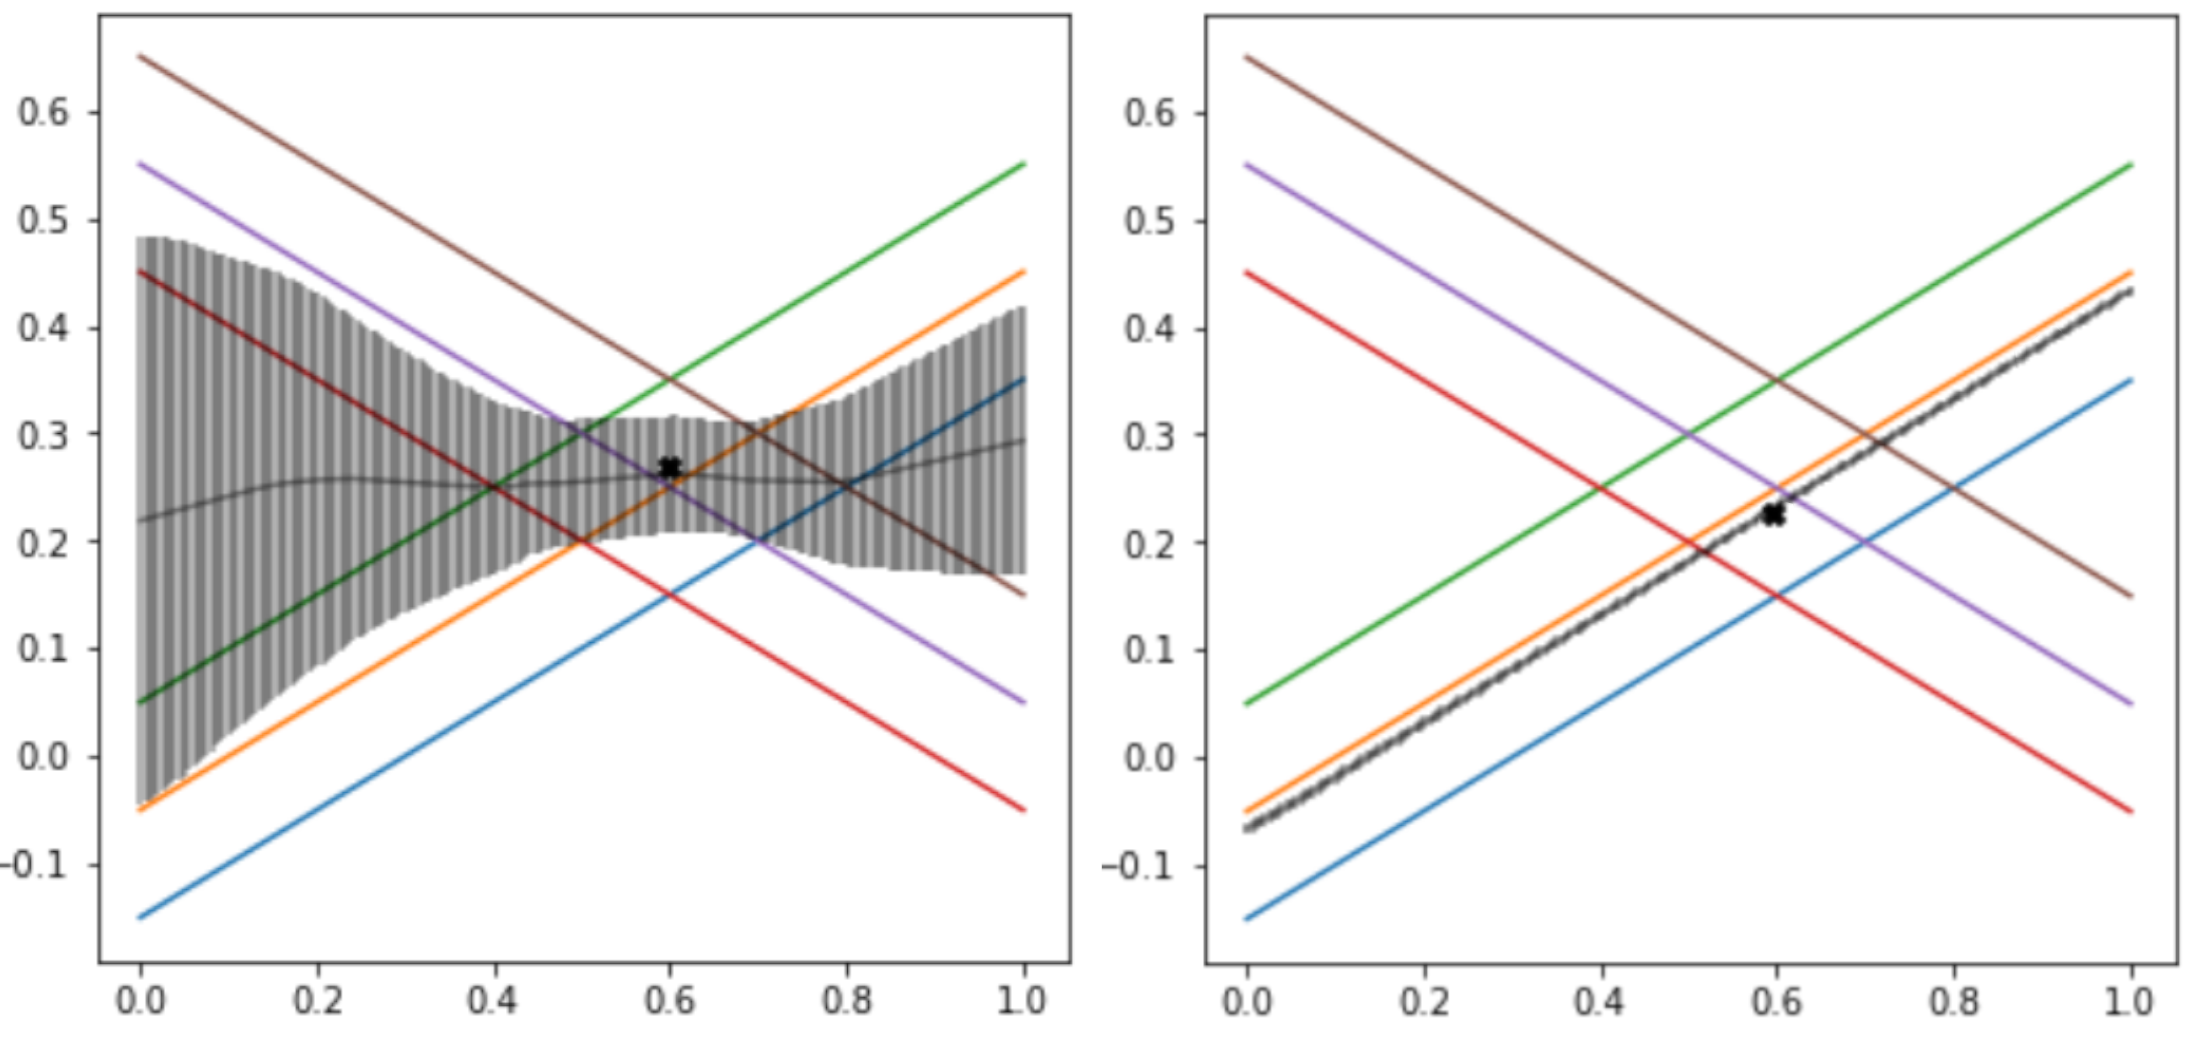
\includegraphics[width=0.8\linewidth]{figures/trajX+tp.png}
    \caption{ CNMP modeling uncertainty for a condition. In the parametrized CNMP, uncertainty is solved, and skills are encoded with task parameters 1 for ascending and 2 for descending. }
    \label{fig:trajX+tp}
\end{figure}

% uncertainty of some observations
The CNMP model is capable of storing different movement primitives of different skills without requiring multiple networks. The selection of the right trajectory is due to the conditioning points (observations) previously explained. The observations are indeed useful for both finding the interpolated trajectory from the demonstrations passing in a new state and also for identifying the correct skill. In \cref{fig:trajX}, the conditioning points identified uniquely the trajectory to generate. However, as it happens in \cref{fig:trajX+tp}, the conditions might be uncertain, so the standard CNMP model averages the outputs, creating a misleading trajectory. 

% introduction TP to eliminate uncertainty
To eliminate uncertainty, a task parameter $\gamma$ (TP) can be included in both the input and the query of the network, as in \cref{fig:cnmp}. The task parameter is a full-fledged new dimension of the network, like input time $t$ and the output value. In the case of the task parameters, the dimension added is an input dimension, which excludes uncertainty. Now, the network, given a condition, can uniquely identify the movement primitive.
\begin{figure}
    \centering
    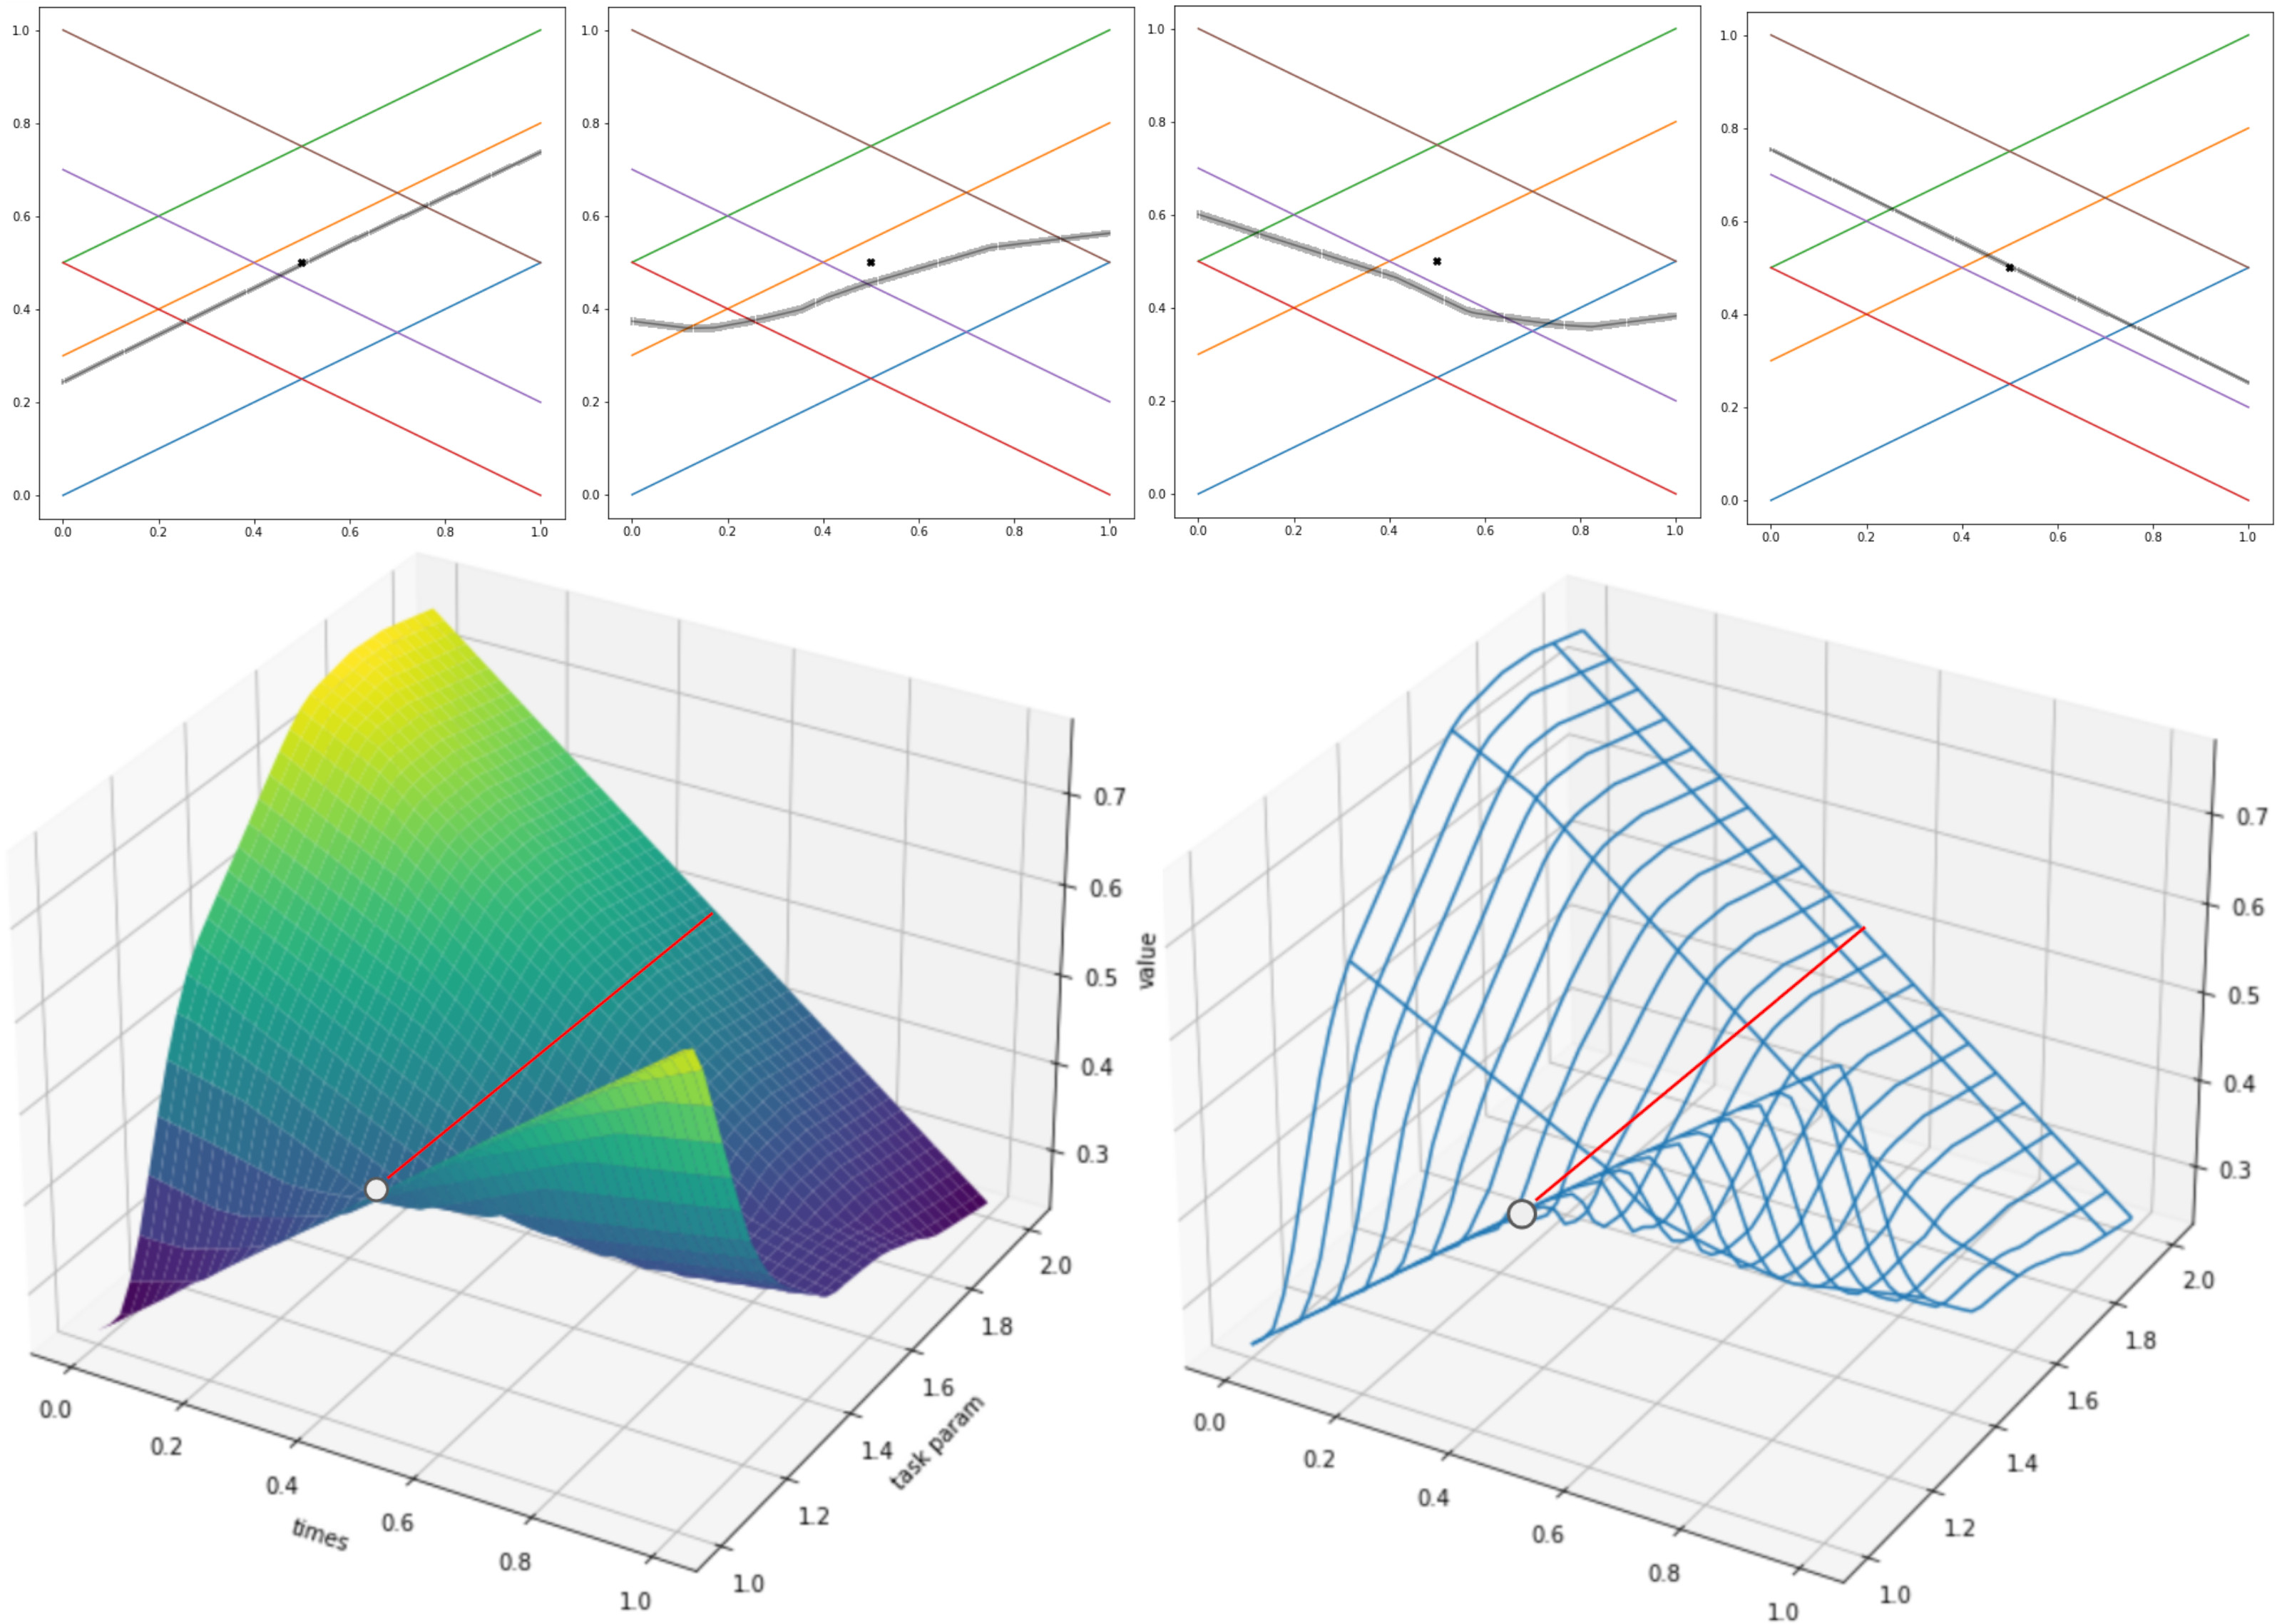
\includegraphics[width=0.9\linewidth]{figures/graph-tp-dimension.jpg}
    \caption{ Plot of the interpolation abilities of CNMPs also in the task-parameter dimension. }
    \label{fig:graph-tp-transition}
\end{figure}
 
% What's among them? (using 1 condition) (shifting) network interpolates nicely
How adding a dimension to the input is interpreted by the networks and what's in between the two parameters has been researched to understand better how to shift among them. In order to do this, a 3D plot is required. This is achieved by leveraging the previously considered weakness of the model of having uncertain conditions. These points are shared by parameters among and maintain the same other dimensions while the external parameter $\gamma$ varies. This doesn't introduce any bias while the condition changes. 

The visualization of a continuous change between different task parameters is present in \cref{fig:graph-tp-transition}. As it's possible to observe, the network interpolates nicely among the functions also in the tasks-parameter space. The movement of the conditioning point in time is depicted in the 3D plot with a red line ending in its final position.

% network has 2 TP, in query and in observation, that varied together
It is worth noting that to obtain the graph in \cref{fig:graph-tp-transition}, both task parameters in the observations and in the query had to vary together. As visible in \cref{fig:cnmp}, the original network design of CNMPs implies the presence of this parameter (as $\gamma$) for the conditioning points and for the query $t$.

% if they don't? difference between observation and query, changing TP
Successively, the difference in variating only one at a time has been researched. In the first place, for all the time steps, only the task parameter of the condition was changed, maintaining the task parameter of the query constant. Next, the opposite was performed to understand how they influence the network result differently.

\begin{figure}
    \centering
    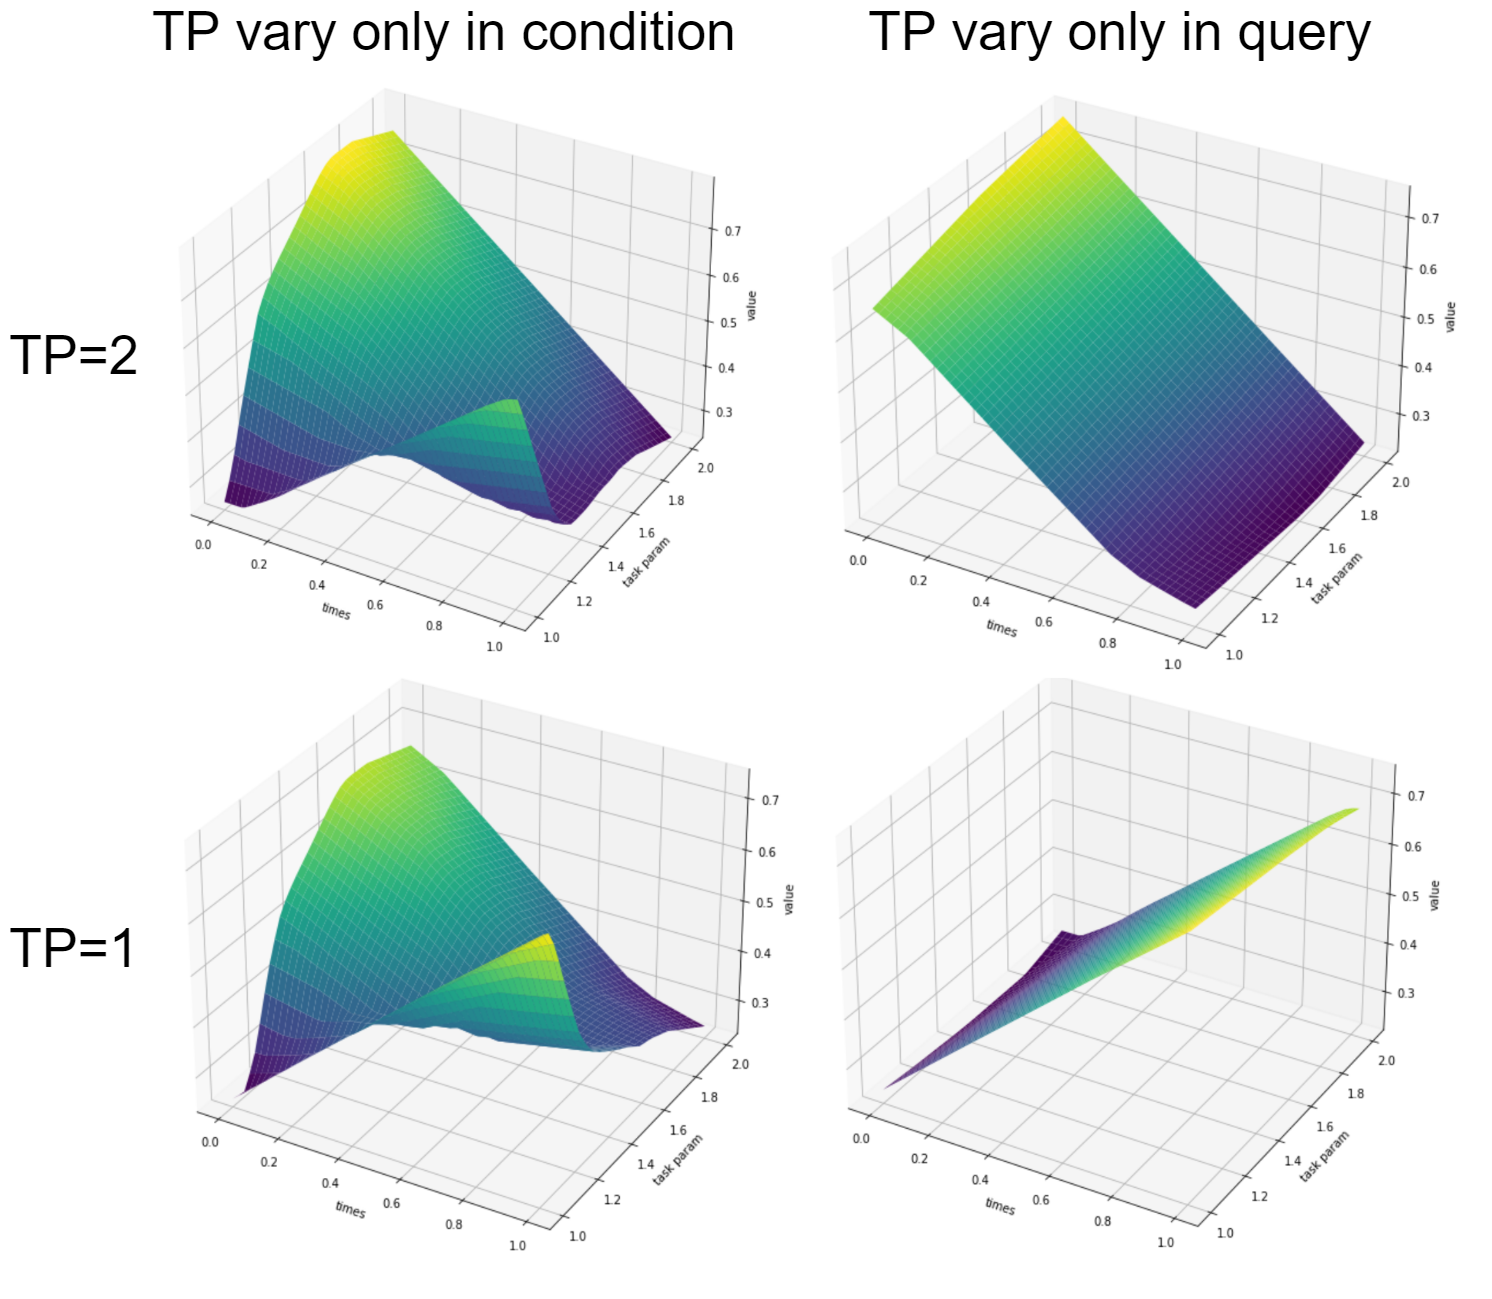
\includegraphics[width=0.8\linewidth]{figures/comparisonCNMPtp-influence.png}
    \caption{ Influence of task parameter from the conditioning points and from the queries. }
    \label{fig:tp-influence}
\end{figure}

The plots comparison is visible in \cref{fig:tp-influence}. On the top row, for task parameter 2, the first graph shows how the result changes according to the variation of the task parameter in the condition. Meanwhile, the second graph shows how, for every time queried, keeping the parameter fixed to 2 in the conditions and changing it in the query doesn't produce a significant variation in the output. 
The second row repeats the procedure with the other task parameter to crosscheck the results. 
It is clearly emerging how the parameter in the observation seems to have a stronger influence than the one in the query, which doesn't seem to contribute significantly. 

The following subsections will investigate the structure of the network and the design of two different architectures. This work proposes before a network with task parameters only in condition and, next, the model with task parameters only in the query. These two architectures are respectively built and examined below.




%%%%%%  Network with only TP in condition  %%%%%%
\subsection{CNMP model with task-parameter only in condition}
This part investigates the architecture of the CNMP model altered to be able to infer the results having the task parameters (TPs) only in the input of the conditions. This design allows querying afterward the network only with the time $t$. 
This architectural choice is motivated by the previous analysis in which the task parameter in the query seemed to have little if no importance for the results. This also feels naturally more sensible for constant tasks as the request is only for the value at a time step, and the task parameter would remain constant anyway. 

\begin{figure}
    \centering
    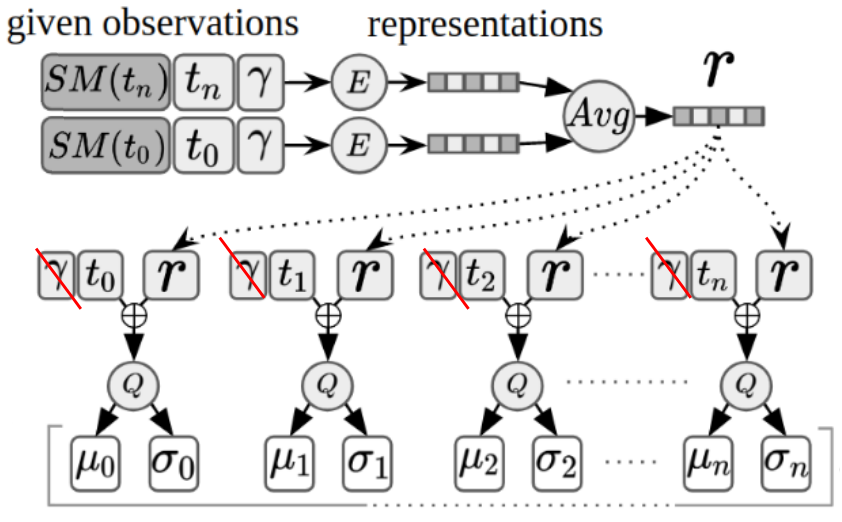
\includegraphics[width=0.7\linewidth]{figures/CNMP_short_no_tp_query.png}
    \caption{ Architecture of the CNMP model proposed without the original task parameter in the queries. }
    \label{fig:CNMP_short_no_tp_query}
\end{figure}

In \cref{fig:CNMP_short_no_tp_query}, the design changes can be compared to the original model. The neural network now feeds the decoder only with the time value to query and the constant representation of the conditions. As a result, the decoder has an input dimension less than the original model.

\begin{longtable}[c]{|c|l|c|c|}
\caption{Comparison Table of errors of original CNMP vs CNMP with TP only in condition}
\label{tab:CNMPvsCNMPnoTPquery}\\
\hline
\textbf{MSE Error} & \textbf{TP} & \textbf{CNMP} & \textbf{CNMP TP condition} \\ \hline
\endfirsthead
\endhead
\multirow{2}{*}{\begin{tabular}[c]{@{}c@{}}on demonstrated\\ trajectory\end{tabular}} & 1 & 2.200240773631327e-06 & 0.0005239668753240399 \\ \cline{2-4} 
 & 2 & 2.852831969051669e-08 & 3.317327413240996e-05 \\ \hline
\multirow{2}{*}{\begin{tabular}[c]{@{}c@{}}on interpolated\\ trajectory\end{tabular}} & 1 & 2.8834989373212024e-06 & 0.0004749418782444545 \\ \cline{2-4} 
 & 2 & 2.598636844065303e-07 & 3.6395583963202646e-06 \\ \hline
\end{longtable}

The new model has been trained on the same dataset and verified with the same validation set.

The quantitative comparison results in \cref{tab:CNMPvsCNMPnoTPquery} show the average mean square errors (MSE) for every task on demonstrated trajectories and interpolated trajectories. The performance of the modified architecture exhibits an increase in the errors that, while present, is not significantly detrimental, suggesting a promising level of robustness in its overall functionality.

The qualitative results of the interpolation can be seen in \cref{fig:comparisonCNMPvsCNMPonlyTPcondition}, and although some interpolation differences are visible, they still clearly maintain a sufficient degree of correctness.

The new network architecture maintains the same interpolation capabilities, but allows the user to query only the time, without worrying about the task parameter, which will be inferred constant from the observations.

\begin{figure}
    \centering
    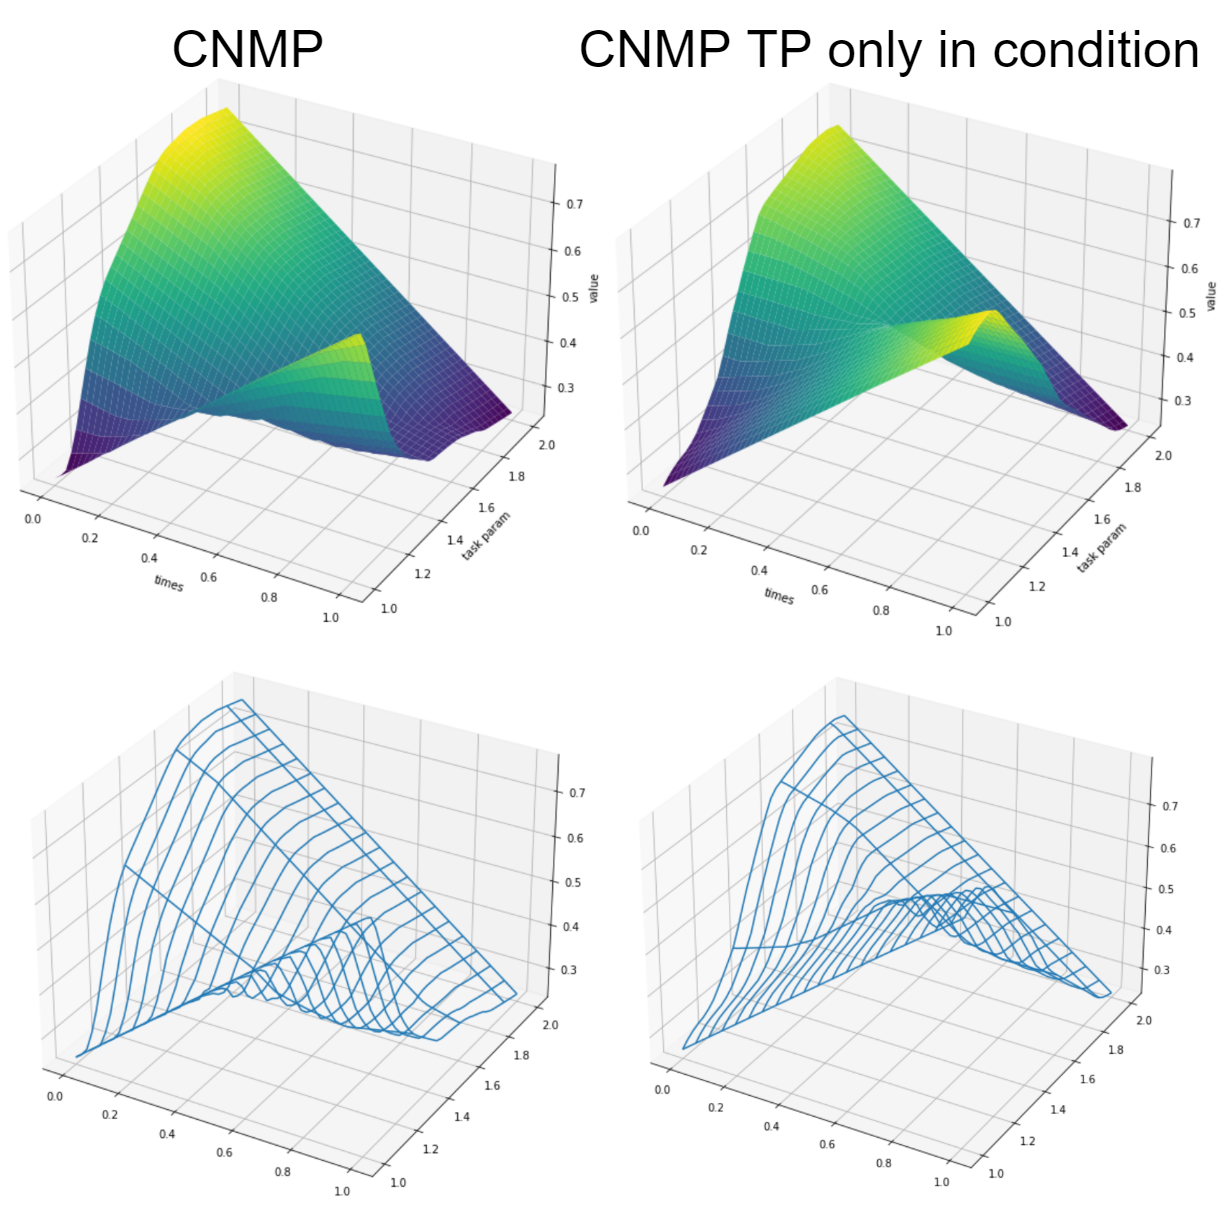
\includegraphics[width=0.8\linewidth]{figures/comparisonCNMPvsCNMPonlyTPcondition.png}
    \caption{ Interpolation comparison of CNMP model vs CNMP model with TP only in the condition. }
    \label{fig:comparisonCNMPvsCNMPonlyTPcondition}
\end{figure}



%%%%%% Network with only TP in query %%%%%%
\subsection{CNMP model with task-parameter only in query}
This subsection analyses the opposite alternative to the previous investigation. The architecture of the CNMP model is altered to generate the results using the task parameters (TPs) only in the input of the query.

This design allows having conditioning points that are parameter-less and querying the network subsequently with the time $t$ and the task parameter $\gamma$. 

This architectural choice seems to be more appropriate for possible changes at run-time of skill by the model. However, it's clearly more challenging since the information is provided later in the pipeline. 

Moreover, conditioning points are responsible for the final position at every time $t$, and feeding the network only subsequently with the task forces it to infer the $\gamma$ of the conditions. 

\begin{figure}
    \centering
    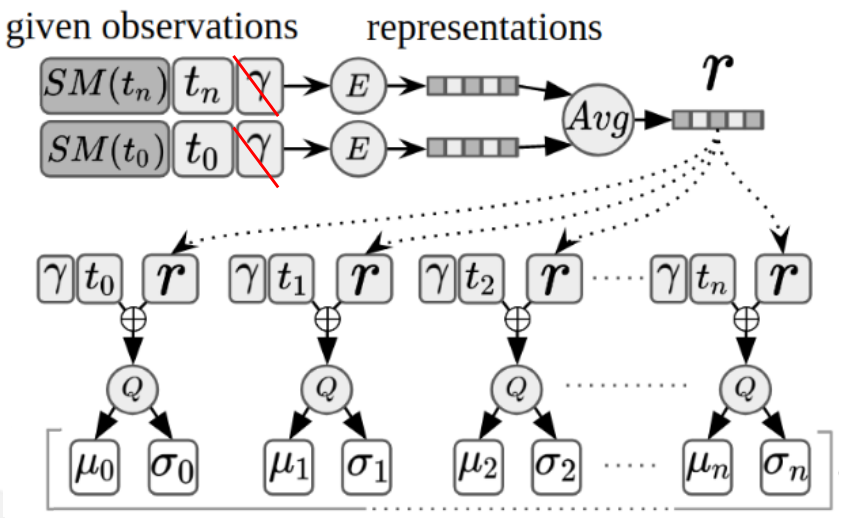
\includegraphics[width=0.7\linewidth]{figures/CNMP_short_no_tp_observations.png}
    \caption{ Architecture of the CNMP model proposed without the original task parameter in the observations. }
    \label{fig:CNMP_short_no_tp_observations}
\end{figure}

In \cref{fig:CNMP_short_no_tp_observations}, the design changes can be compared to the original model. The neural network now feeds the encoder with observations that don't have any parameter, delaying the $\gamma$ inference to the decoder. As a result, the encoder has an input dimension less than the original model.

The second new model has been trained on the same dataset and verified with the same validation set as the previously discussed ones.

\begin{longtable}[c]{|c|l|c|l|}
\caption{Comparison Table of errors of original CNMP vs CNMP with TP only in query}
\label{tab:CNMPvsCNMPnoTPcondition}\\
\hline
\textbf{MSE Error} & \textbf{TP} & \textbf{CNMP} & \multicolumn{1}{c|}{\textbf{CNMP TP query}} \\ \hline
\endfirsthead
%
\endhead
%
\multirow{2}{*}{\begin{tabular}[c]{@{}c@{}}on demonstrated\\ trajectory\end{tabular}} & 1 & 2.200240773631327e-06 & 0.00015134105003480186 \\ \cline{2-4} 
 & 2 & 2.852831969051669e-08 & 1.5758800492775196e-05 \\ \hline
\multirow{2}{*}{\begin{tabular}[c]{@{}c@{}}on interpolated\\ trajectory\end{tabular}} & 1 & 2.8834989373212024e-06 & 0.0008166800702431865 \\ \cline{2-4} 
 & 2 & 2.598636844065303e-07 & 0.0002007523980230904 \\ \hline
\end{longtable}


The quantitative comparison results in \cref{tab:CNMPvsCNMPnoTPcondition} show the average mean square errors (MSE) for every task on demonstrated trajectories and interpolated trajectories. The modified architecture again demonstrates a rise in errors compared to the original model, but these errors, though now noticeable, do not compromise the usability of the model.
\begin{figure}
    \centering
    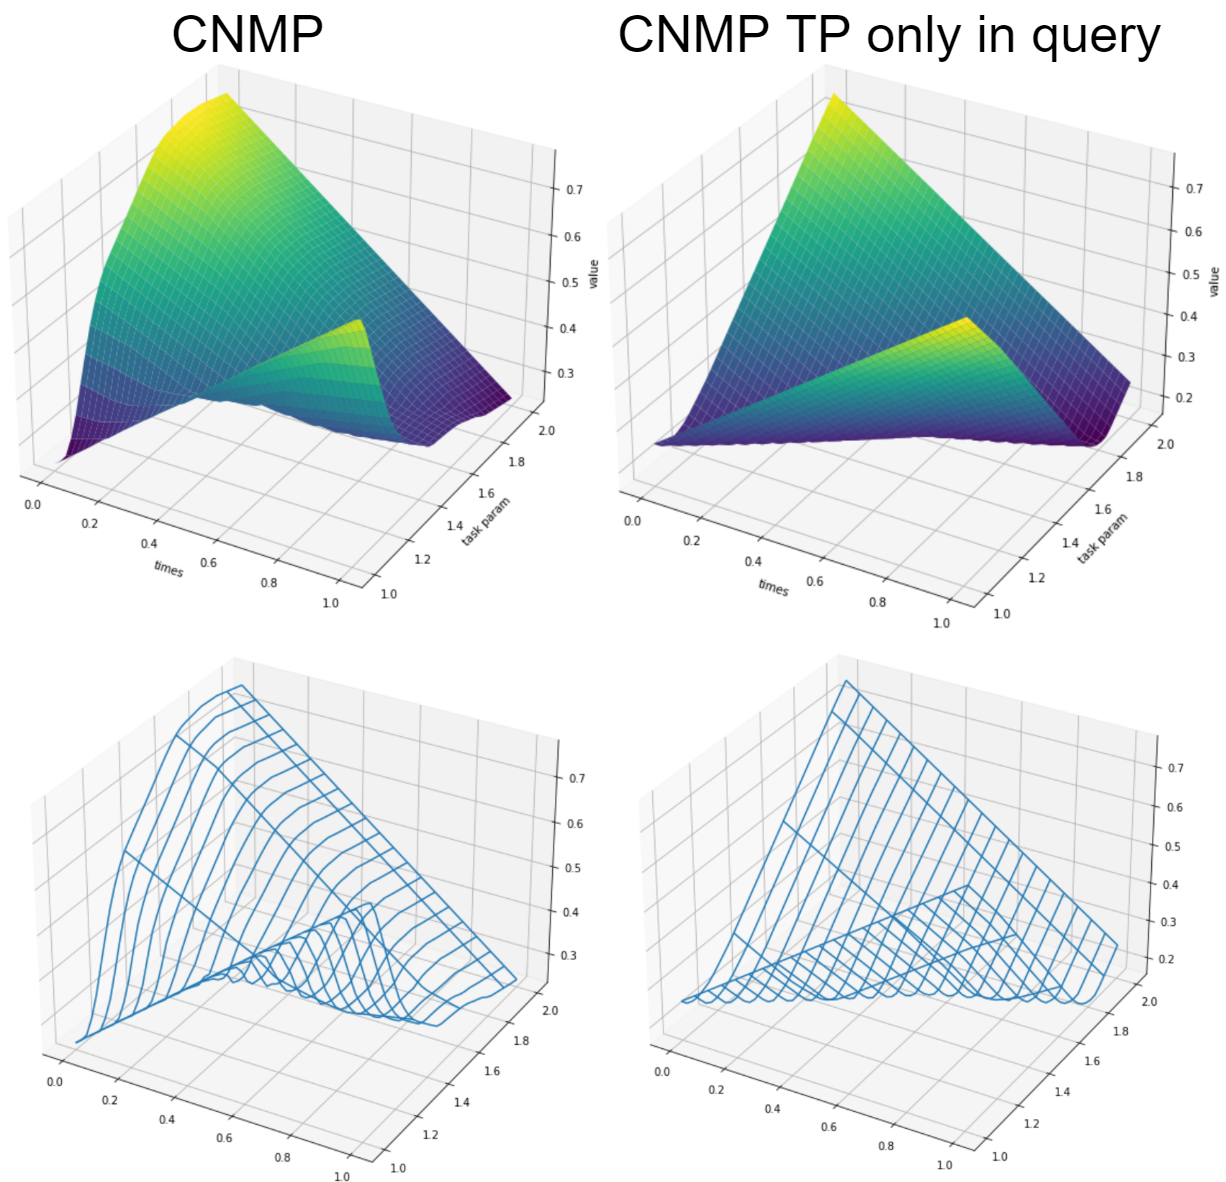
\includegraphics[width=0.8\linewidth]{figures/comparisonCNMPvsCNMPonlyTPquery.png}
    \caption{ Interpolation comparison of CNMP model vs CNMP model with TP only in the query. }
    \label{fig:comparisonCNMPvsCNMPonlyTPquery}
\end{figure}
Not the same can be said for the qualitative results of the interpolation. The comparison that can be seen in \cref{fig:comparisonCNMPvsCNMPonlyTPquery} shows a remarkable drop in the values in the interpolated area between the two functions. This will clearly impact the correctness of a transition among them. The inaccuracy is probably due to the fact that the parameter information goes through an inferior network depth compared to the full model.  
Nevertheless, these results leave room for further research on how to condition with one state parameterless and let the network, queried with different tasks, pass through that state.




%%%%%% Comparison %%%%%%
\subsection{Comparison of the previous models}
A comparison of the three previously discussed models is presented below to better evaluate the most capable and cross-validate the results. 
A different dataset was built with different parametric functions: linear, parabolic, and sinusoidal. This also implies the presence of three different tasks to feed to a single CNMP network. For each skill, different trajectories are present in the dataset to enable new trajectory generation for conditioning points of unseen values. 

Moreover, the transition among all tasks is now represented with three values, so the first task is encoded as $[1][0][0]$, the second as $[0][1][0]$, the third as $[0][0][1]$. This avoids passing through the middle one as in the case of a single parameter $[1..2..3]$ encoded network. The transition is performed by decreasing one value and increasing the other simultaneously.

\begin{longtable}[c]{|c|l|c|c|l|}
\caption{Full Comparison Table of errors of CNMP vs CNMP with TP only in condition vs CNMP with TP only in query}
\label{tab:CNMP3vs}\\
\hline
\textbf{\begin{tabular}[c]{@{}c@{}}MSE Error \\on \end{tabular}} & \textbf{TP} & \textbf{CNMP} & \textbf{\begin{tabular}[c]{@{}c@{}}CNMP \\ TP condition\end{tabular}} & \multicolumn{1}{c|}{\textbf{\begin{tabular}[c]{@{}c@{}}CNMP \\ TP query\end{tabular}}} \\ \hline
\endfirsthead
%
\endhead
%
\multirow{2}{*}{\begin{tabular}[c]{@{}c@{}}demonstrated\\ trajectory\end{tabular}} & 1 & 2.200240773e-06 & 0.0005239668753 & 0.00015134105003 \\ \cline{2-5} 
 & 2 & 2.852831969e-08 & 3.317327413e-05 & 1.5758800492e-05 \\ \hline
\multirow{2}{*}{\begin{tabular}[c]{@{}c@{}}interpolated\\ trajectory\end{tabular}} & 1 & 2.8834989373e-06 & 0.0004749418782 & 0.0008166800702 \\ \cline{2-5} 
 & 2 & 2.598636844e-07 & 3.6395583963e-06 & 0.0002007523980 \\ \hline
\end{longtable}

In \cref{fig:comparisonCNMP3trajectories}, it is possible to observe all the possible combinations for interpolating the different tasks on which the network has been trained. Even with more than two tasks and three dimensions added to the input the CNMP model performs sufficiently well in all three skills. 

\begin{figure}
    \centering
    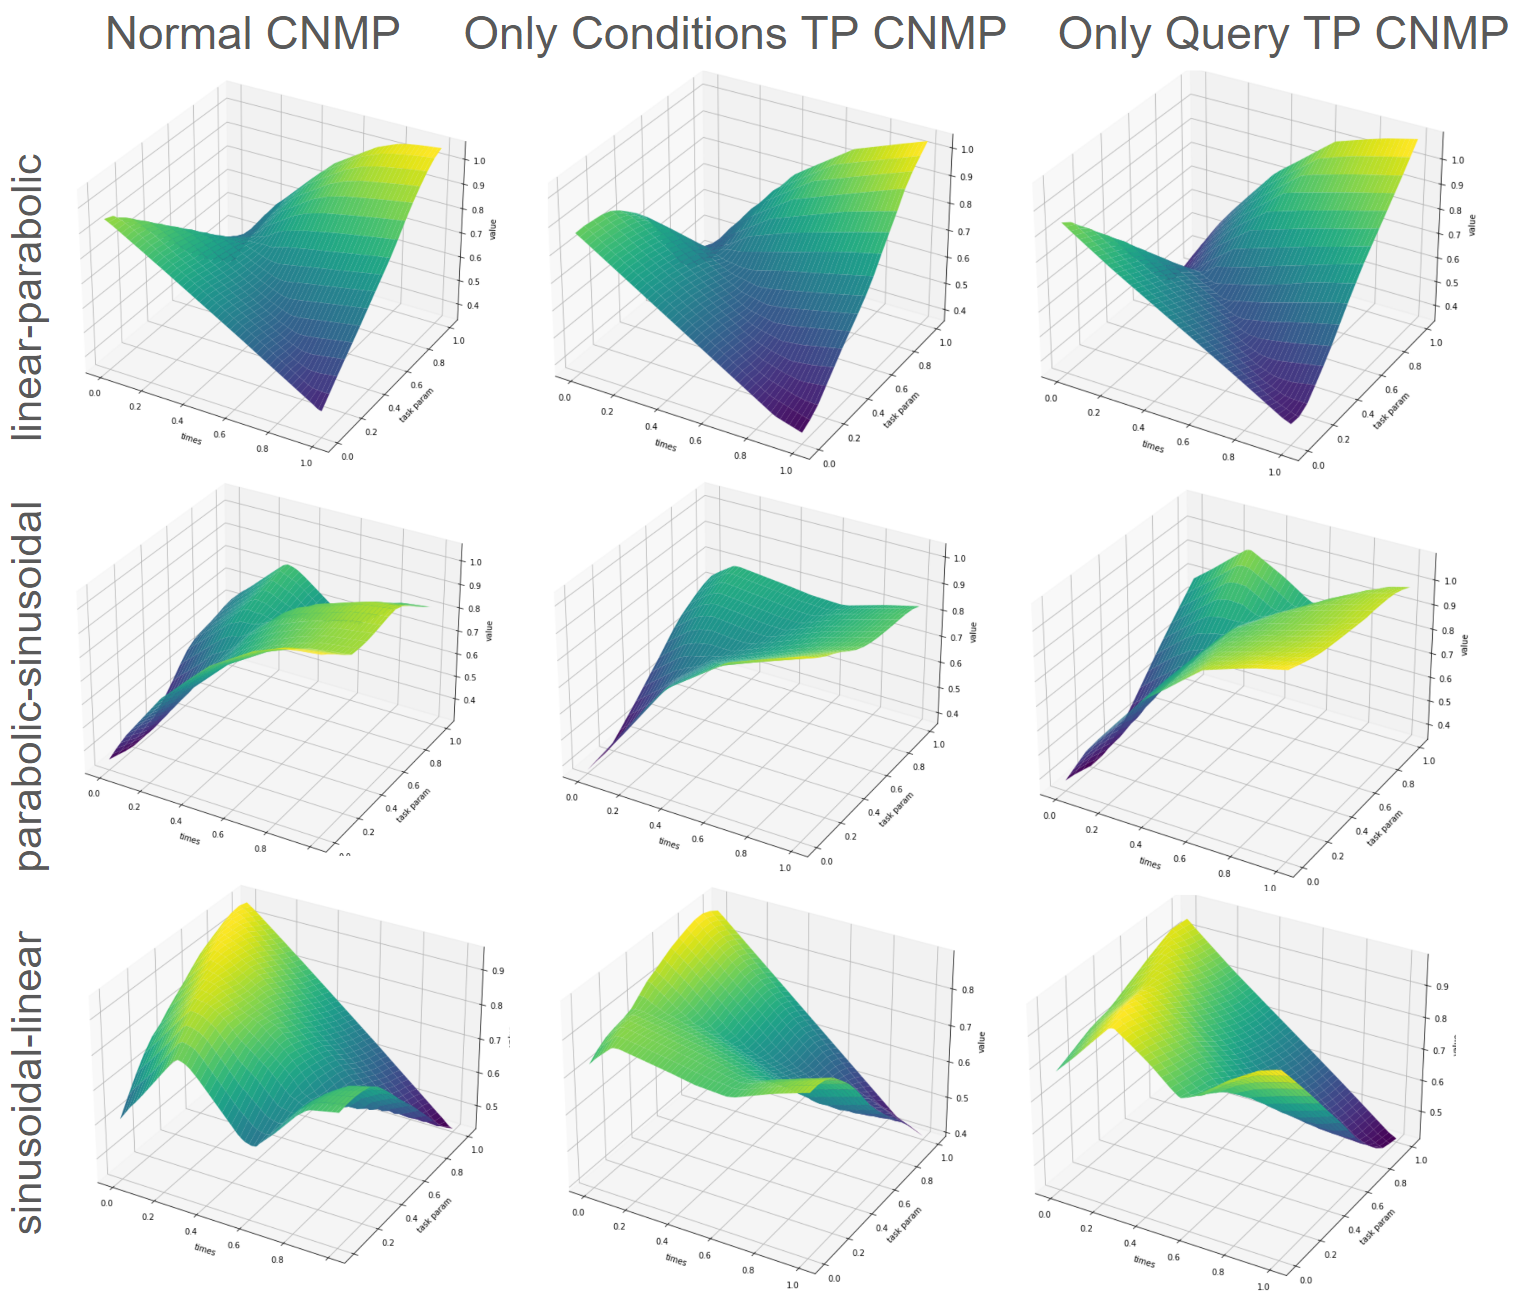
\includegraphics[width=0.9\linewidth]{figures/comparisonCNMP3trajectories.png}
    \caption{ Interpolation comparison of the 3 CNMP models analyzed for a different dataset and multiple tasks. }
    \label{fig:comparisonCNMP3trajectories}
\end{figure}


\newpage
%%%%%% shifting TP in time with 1 condition %%%%%%
\subsection{CNMP changing task in time with one conditioning point}
Analyzed the interpolation capabilities of the CNMP networks also on the task dimension, a possible method to shift the execution of a skill in time is proposed below. 

In order to build the interpolation visualizations, the network was always queried for every time-step with a constant $\gamma$. 
However, since the queries are independent, it's possible to query the time and parameter singularly as required.

Moreover, from the previously constructed plots, it is evident how it is possible to change tasks in time via querying the network with TPs linearly changing with time.

\begin{figure}
    \centering
    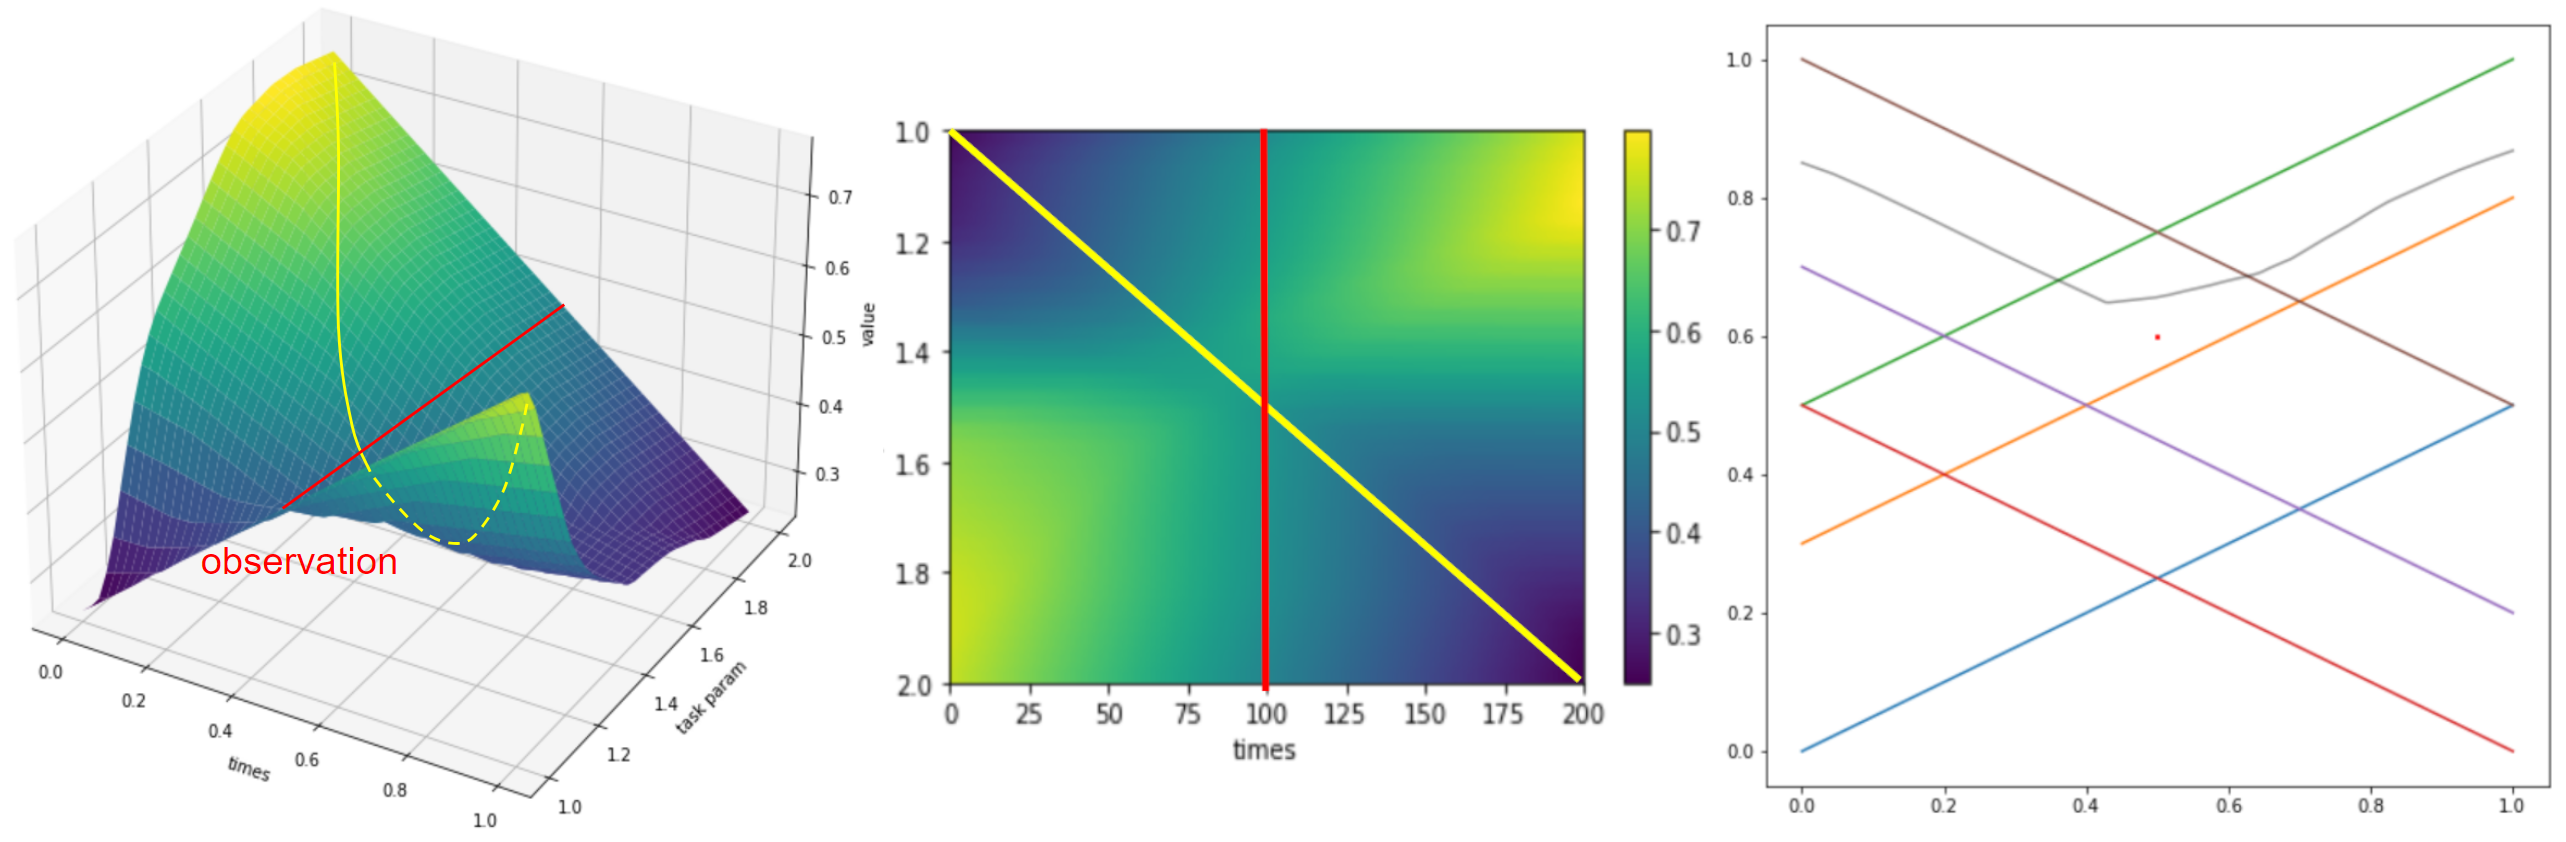
\includegraphics[width=0.95\linewidth]{figures/tpshift.png}
    \caption{ Transition in time of task through task parameter shifting }
    \label{fig:tpshift}
\end{figure}

In \cref{fig:tpshift}, the path of the queries of time and $\gamma$ is depicted in yellow. As time goes on, left to right, the action moves from descending (back of the graph) to ascending (front of the graph). This achieves a smooth change between task parameters using the interpolation space provided by the model. 

In this case, math leverages the neural network's hidden capabilities to wisely input the required parameters to generate the desired output. 

It's worth noting that this method works with any CNMP model variation previously discussed, as long as the interpolation space is built correctly. Further research could include better training to improve the results in the interpolation dimensions.  

The mixing of the two different skills is indeed performed through time, and in this case, the change is linear. Different functions analyzed produced different results, among them the most famous ones like sigmoid, logarithmic, and others. The model is capable of different transition speeds and periods depending on the selected function. The linear function is selected given that it produces the smoothest transitions since inclination is minimal in all the timesteps. 

On the opposite, a sharper function, like a step function in \cref{fig:tpshift-diff-functions}, produces a shift that is immediate and full-fledged a stitch among two parts. 

\begin{figure}
    \centering
    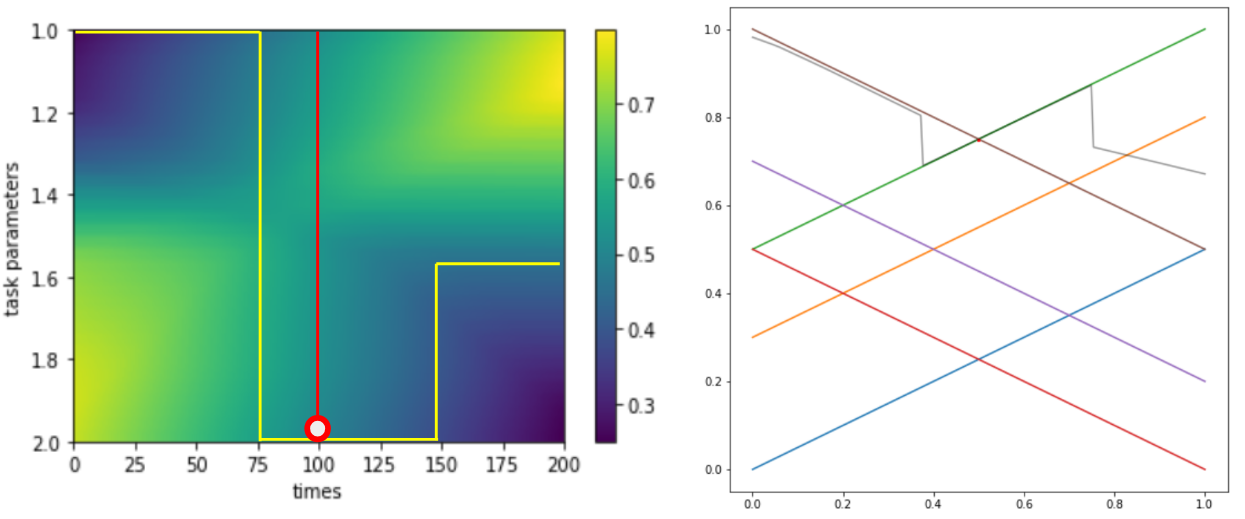
\includegraphics[width=0.8\linewidth]{figures/tpshift-diff-functions.png}
    \caption{ Different functions for changing task parameter in the CNMP network }
    \label{fig:tpshift-diff-functions}
\end{figure}

% 1 condition position discussion
In \cref{fig:tpshift}, it is possible to see that the final trajectory result is not passing through the conditioning point. This occurs since, at that moment $t=0.5$, the transition between two different task parameters is halfway ($\gamma=1.5$) and not fully on one $\gamma$. The interpolated space varies in quality depending on the network and its training, and this means the error would be higher compared to the values on $\gamma$ on which the model was trained. 

Surprisingly, it's not actually a problem because the conditioning point is nothing else than a point that symbolizes the transition between two conditioning points with different $\gamma$ located on different positions. The conditioning point is just a point that allows the transition without introducing any bias because it's part of both trajectories. In \cref{fig:tp-condition-point-meaning}, it is possible to see the red conditioning point emulating two different conditions with different TP, respectively descending for the left one and ascending for the right one.

This means that the conditioning point for transition is not meant to be anywhere, but it has to be at the intersection of the two desired functions with different TPs. This will grant the resulting function to pass at the initial time through the first conditioning point, since its TP is not mixed, and at the final time through the second condition for the same reason. 

In the example \cref{fig:tp-condition-point-meaning}, at time $t=0$, the function passes through the first point because the task parameter is fully descending. This is guaranteed because the red observation chosen is on the line produced by that initial point. In the same way, at time $t=1$, it's guaranteed to pass through the rightmost point because the observation is also on the function that is produced by that condition. 
For this reason, the observation point is not meant to be independent but derived from the two points to emulate.

\begin{figure}
    \centering
    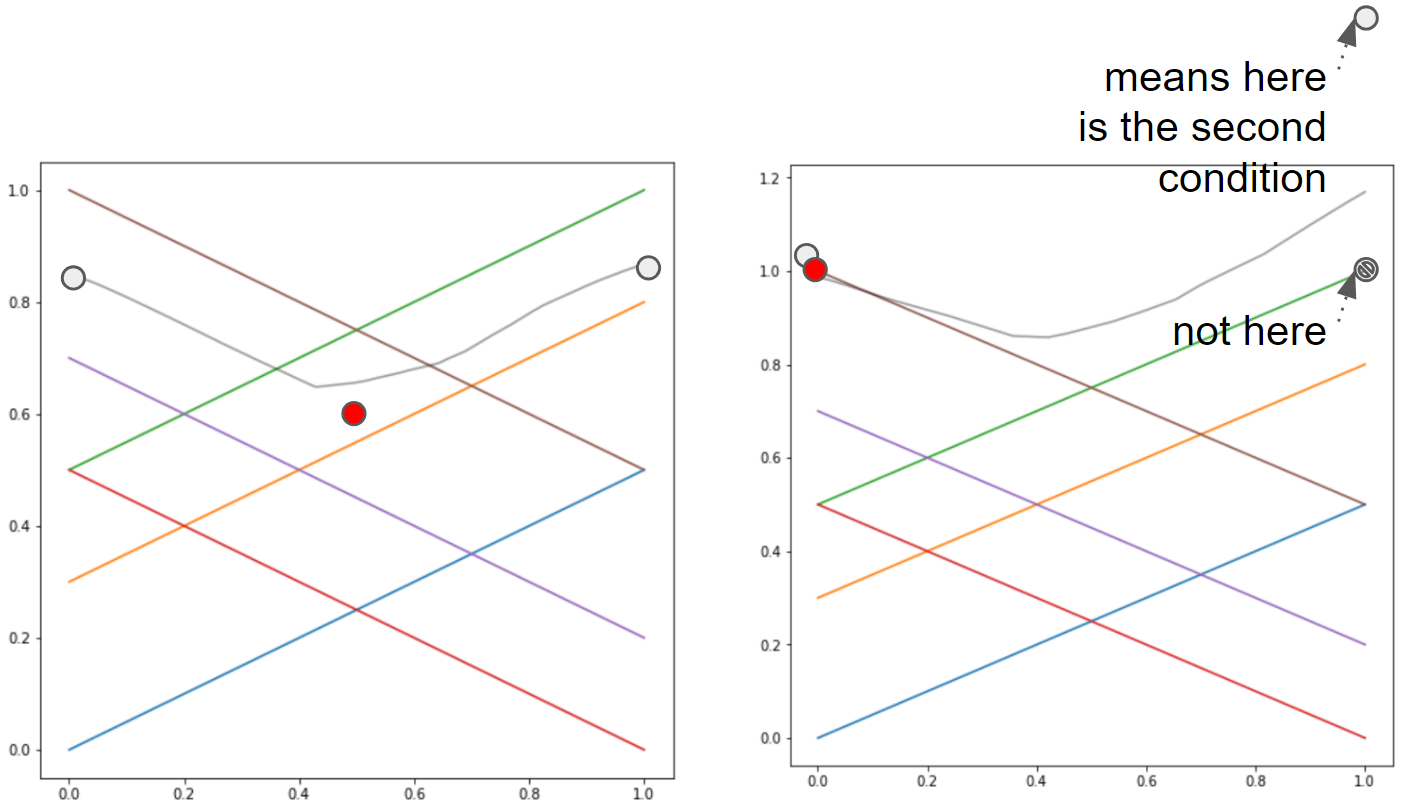
\includegraphics[width=0.8\linewidth]{figures/tp-condition-point-meaning.png}
    \caption{ A conditioning point that varies task parameter emulates two different conditioning points of different task parameters. }
    \label{fig:tp-condition-point-meaning}
\end{figure}

The best strategy to find the conditioning point for the transition among two conditions of different $\gamma$ seems to place it on the intersection of the two trajectories generated by these conditions. However, it is not always granted that the trajectories will intersect. As discussed above, in multidimensional spaces, the probability of this event decreases significantly. 

When two functions don't intersect, the best possible solution to not bias the interpolation is, while changing the $\gamma$, to shift as well the position of the condition in time. In the series of queries to the network, instead of giving the same context point and changing its task parameter, the position also changes. The optimal change of position is from a point on the first function generated by the first condition to the closest point on the function generated by the second condition. This guarantees the series of points will stay on the interpolation of the two functions and generate the desired interpolation surface area.

Extending the concept, the algorithm defined looks for the closest points among the two functions, and it transitions among them. 
The closest couple of points is looked only in the time span in which the network was trained, since it is a computation of cost $t^2$.
If there is an intersection, the change on the conditioning point will be only on the task parameter. 
If there is no intersection, the change of the conditioning point will also be a change in position from the closest point of the first function to the closest of the second one.


%%%%%% shifting TP in time with multiple conditions  %%%%%%
\subsection{CNMP changing task in time with multiple conditioning points}
The system developed enables a single transition using a single conditioning point. The shift occurs completely from an initial time that is $t=0$ to the final time of the network training.

It's a remarkable success because the bare normal CNMP model is completely incapable of changing the task coherently and continuously among its predictions. 
If fed with two conditions of different TP, the network outputs a completely unusable trajectory. This trajectory is a rough average of all the different ones generated by the conditioning points. This is due to the fact that the model, by definition, doesn't have an attention mechanism and doesn't lose the conditioning power in time.

However, this research extends the method further to multiple conditions with different task parameters. This enables the full control and customization of the predicted output. 

Furthermore, it achieves the shift among the observations in a desired time span not restricted to the full training time length. 

Once the interpolated surface is built, the time constraints are resolved with a fast transition from the first condition timestep to the second condition timestep. The resulting output sequence will still reside on the interpolated surface but, having less time, will be faster.

\begin{figure}
    \centering
    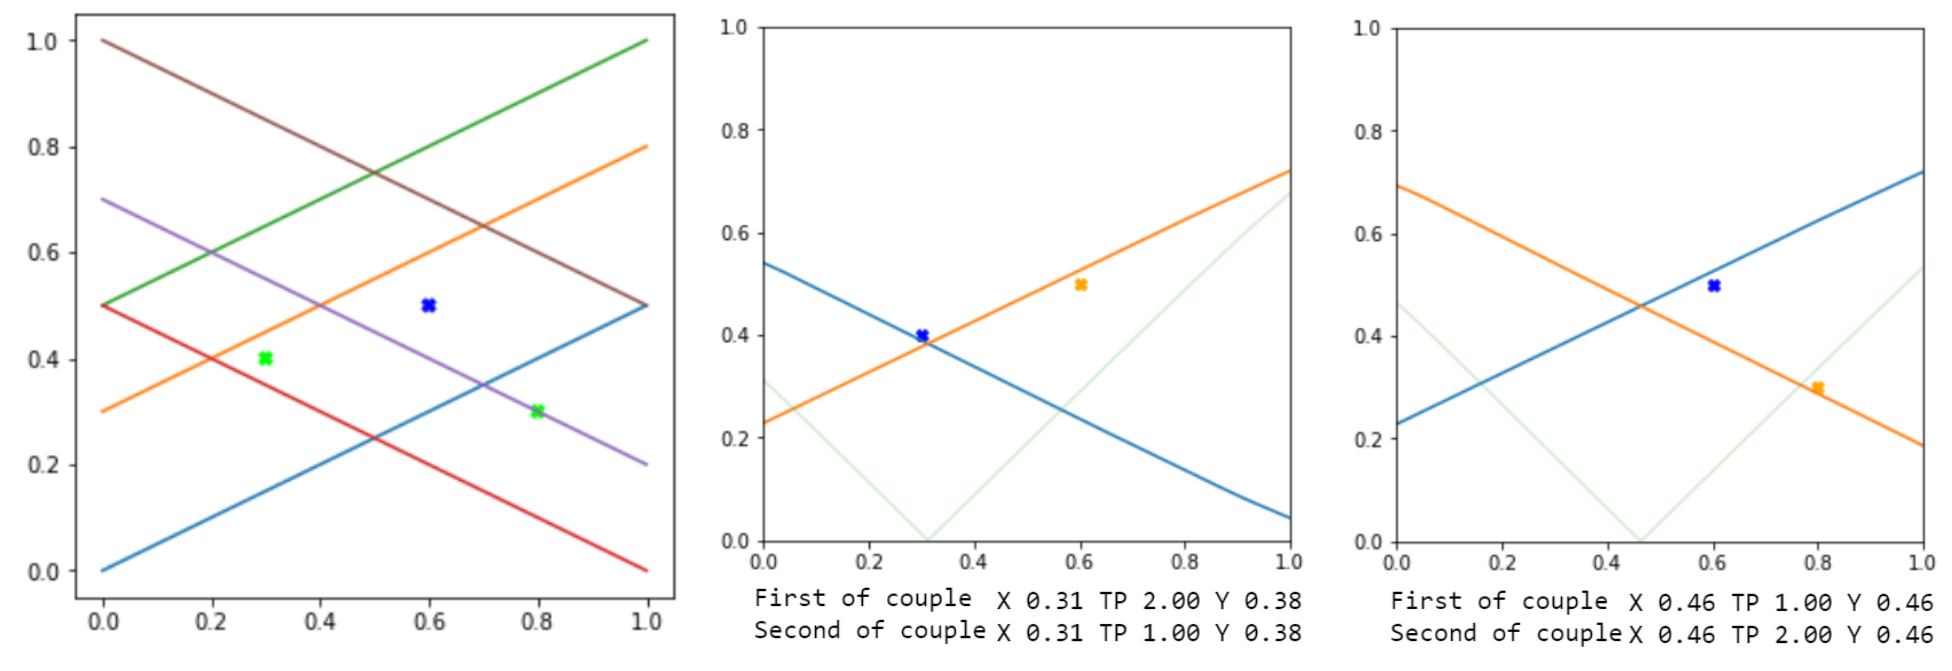
\includegraphics[width=0.95\linewidth]{figures/tp-multiple-shift.png}
    \caption{ Procedure to individuate multiple conditions for multiple shifts in the task parameters. }
    \label{fig:tp-multiple-shift}
\end{figure}

The multiple transitions are achieved by coupling them one by one in temporal order, so the first one determines the task parameter till its time. Then, between the first and the second one, the task is shifted. At the second observation, the task parameter will be fully on its task, but subsequently, will start to be merged with the third one, and so on. This guarantees that at the observation's times, the output function will pass through them, but in between, the task change will occur.  

In \cref{fig:tp-multiple-shift}, it is possible to view the initial observations of different parameters, two green conditioning points for the descending task and one blue in the middle for the ascending task. The first couple in temporal order is selected. At this point, the two functions each condition will independently create are generated. Those are visible in the \cref{fig:tp-multiple-shift} in the second plot. 

The closest points between these functions are selected, the absolute distance among the points is plotted as the green line at the bottom of the plot. In this case, since there is an intersection, the couple selected has the same starting and ending position, which only differs for the $\gamma$ parameter. During the shift time, the conditioning point of the network will transition from the first identified to the other one, changing TP. If the two closest points were in different locations, it would also change location, along with task parameter. 
The network is queried at the appropriate time with the condition designated.

\begin{figure}
    \centering
    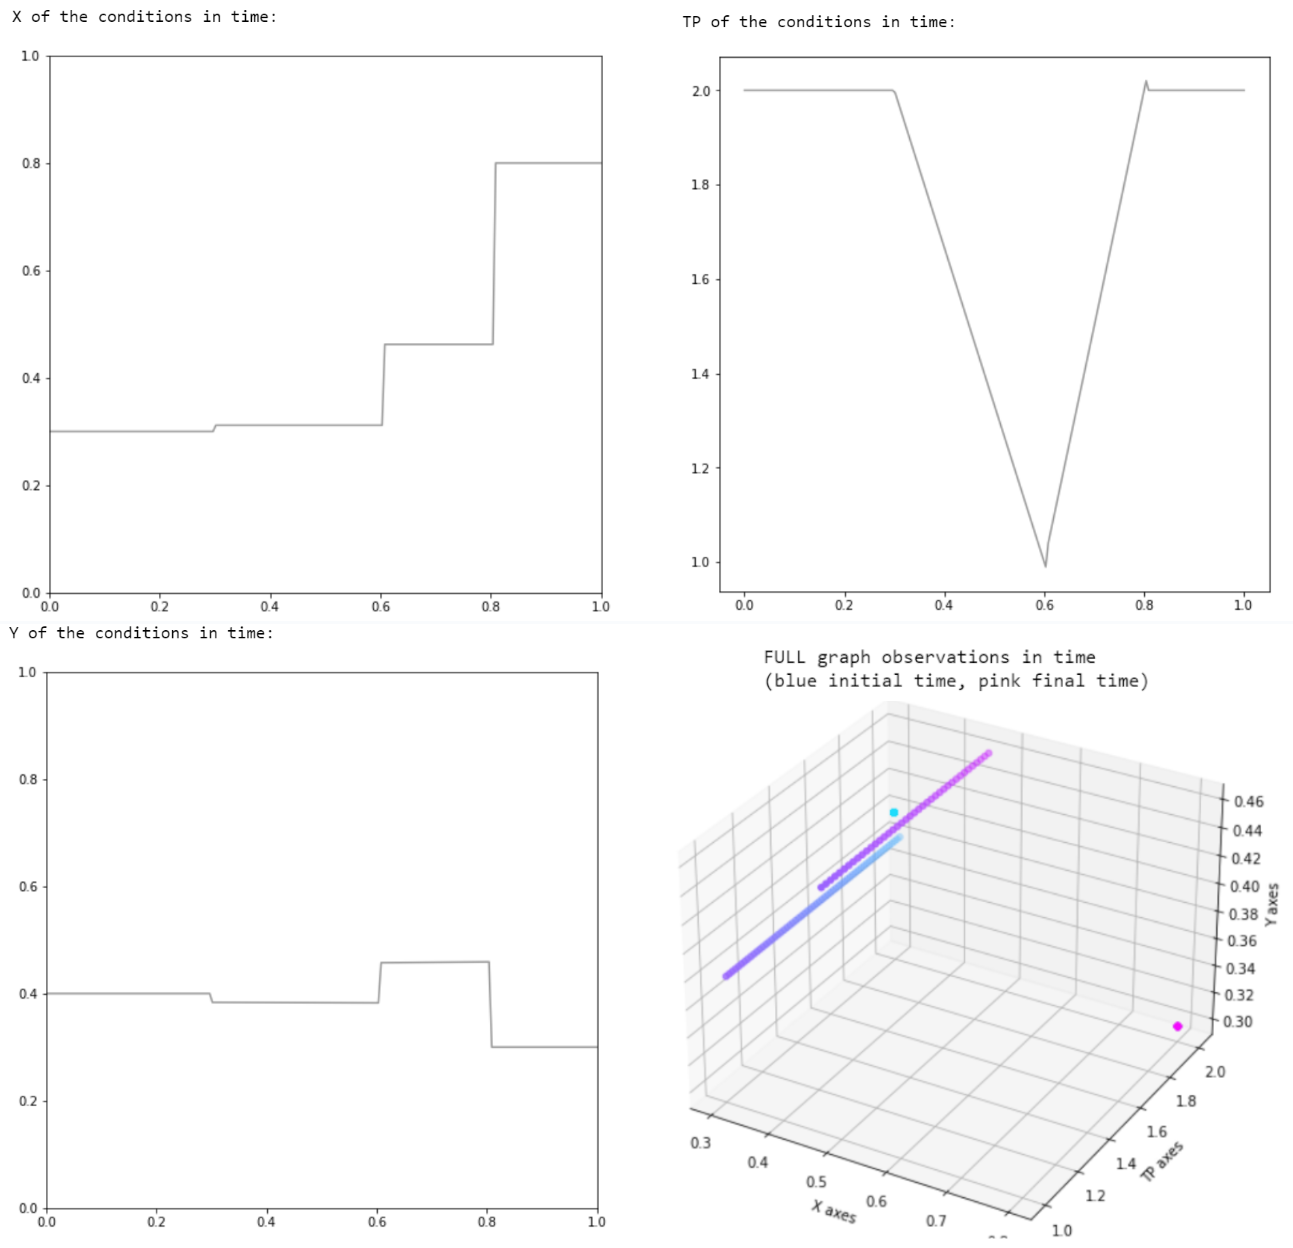
\includegraphics[width=0.7\linewidth]{figures/tp-multiple-shift-condition.png}
    \caption{ Graph and full path in time of the condition point used to transition multiple tasks parameters }
    \label{fig:tp-multiple-shift-condition}
\end{figure}


The process repeats for the second couple and so on to find the conditioning points to feed the network to obtain the desired result. 
The final full path of the conditioning point is visible in \cref{fig:tp-multiple-shift-condition} where it changes position in time according to the place where it will not bias the current transition. Meanwhile, the changing of the TP will occur during the time span designated.

It's worth noting that the conditioning point will also change its time, independently from the time queried. For this reason, in the 3D graph in \cref{fig:tp-multiple-shift-condition} the fourth dimension is introduced as color. The x axes of the graph corresponds now to the time of the condition, while the time of the queries corresponds to the change in color. 

Finally, the results shown in \cref{fig:tp-multiple-shift-results} demonstrate how this method can achieve trajectory predictions that are coherent across multiple shifts of tasks. The normal CNMP model with the same conditioning points is reported aside for comparison. 

\begin{figure}
    \centering
    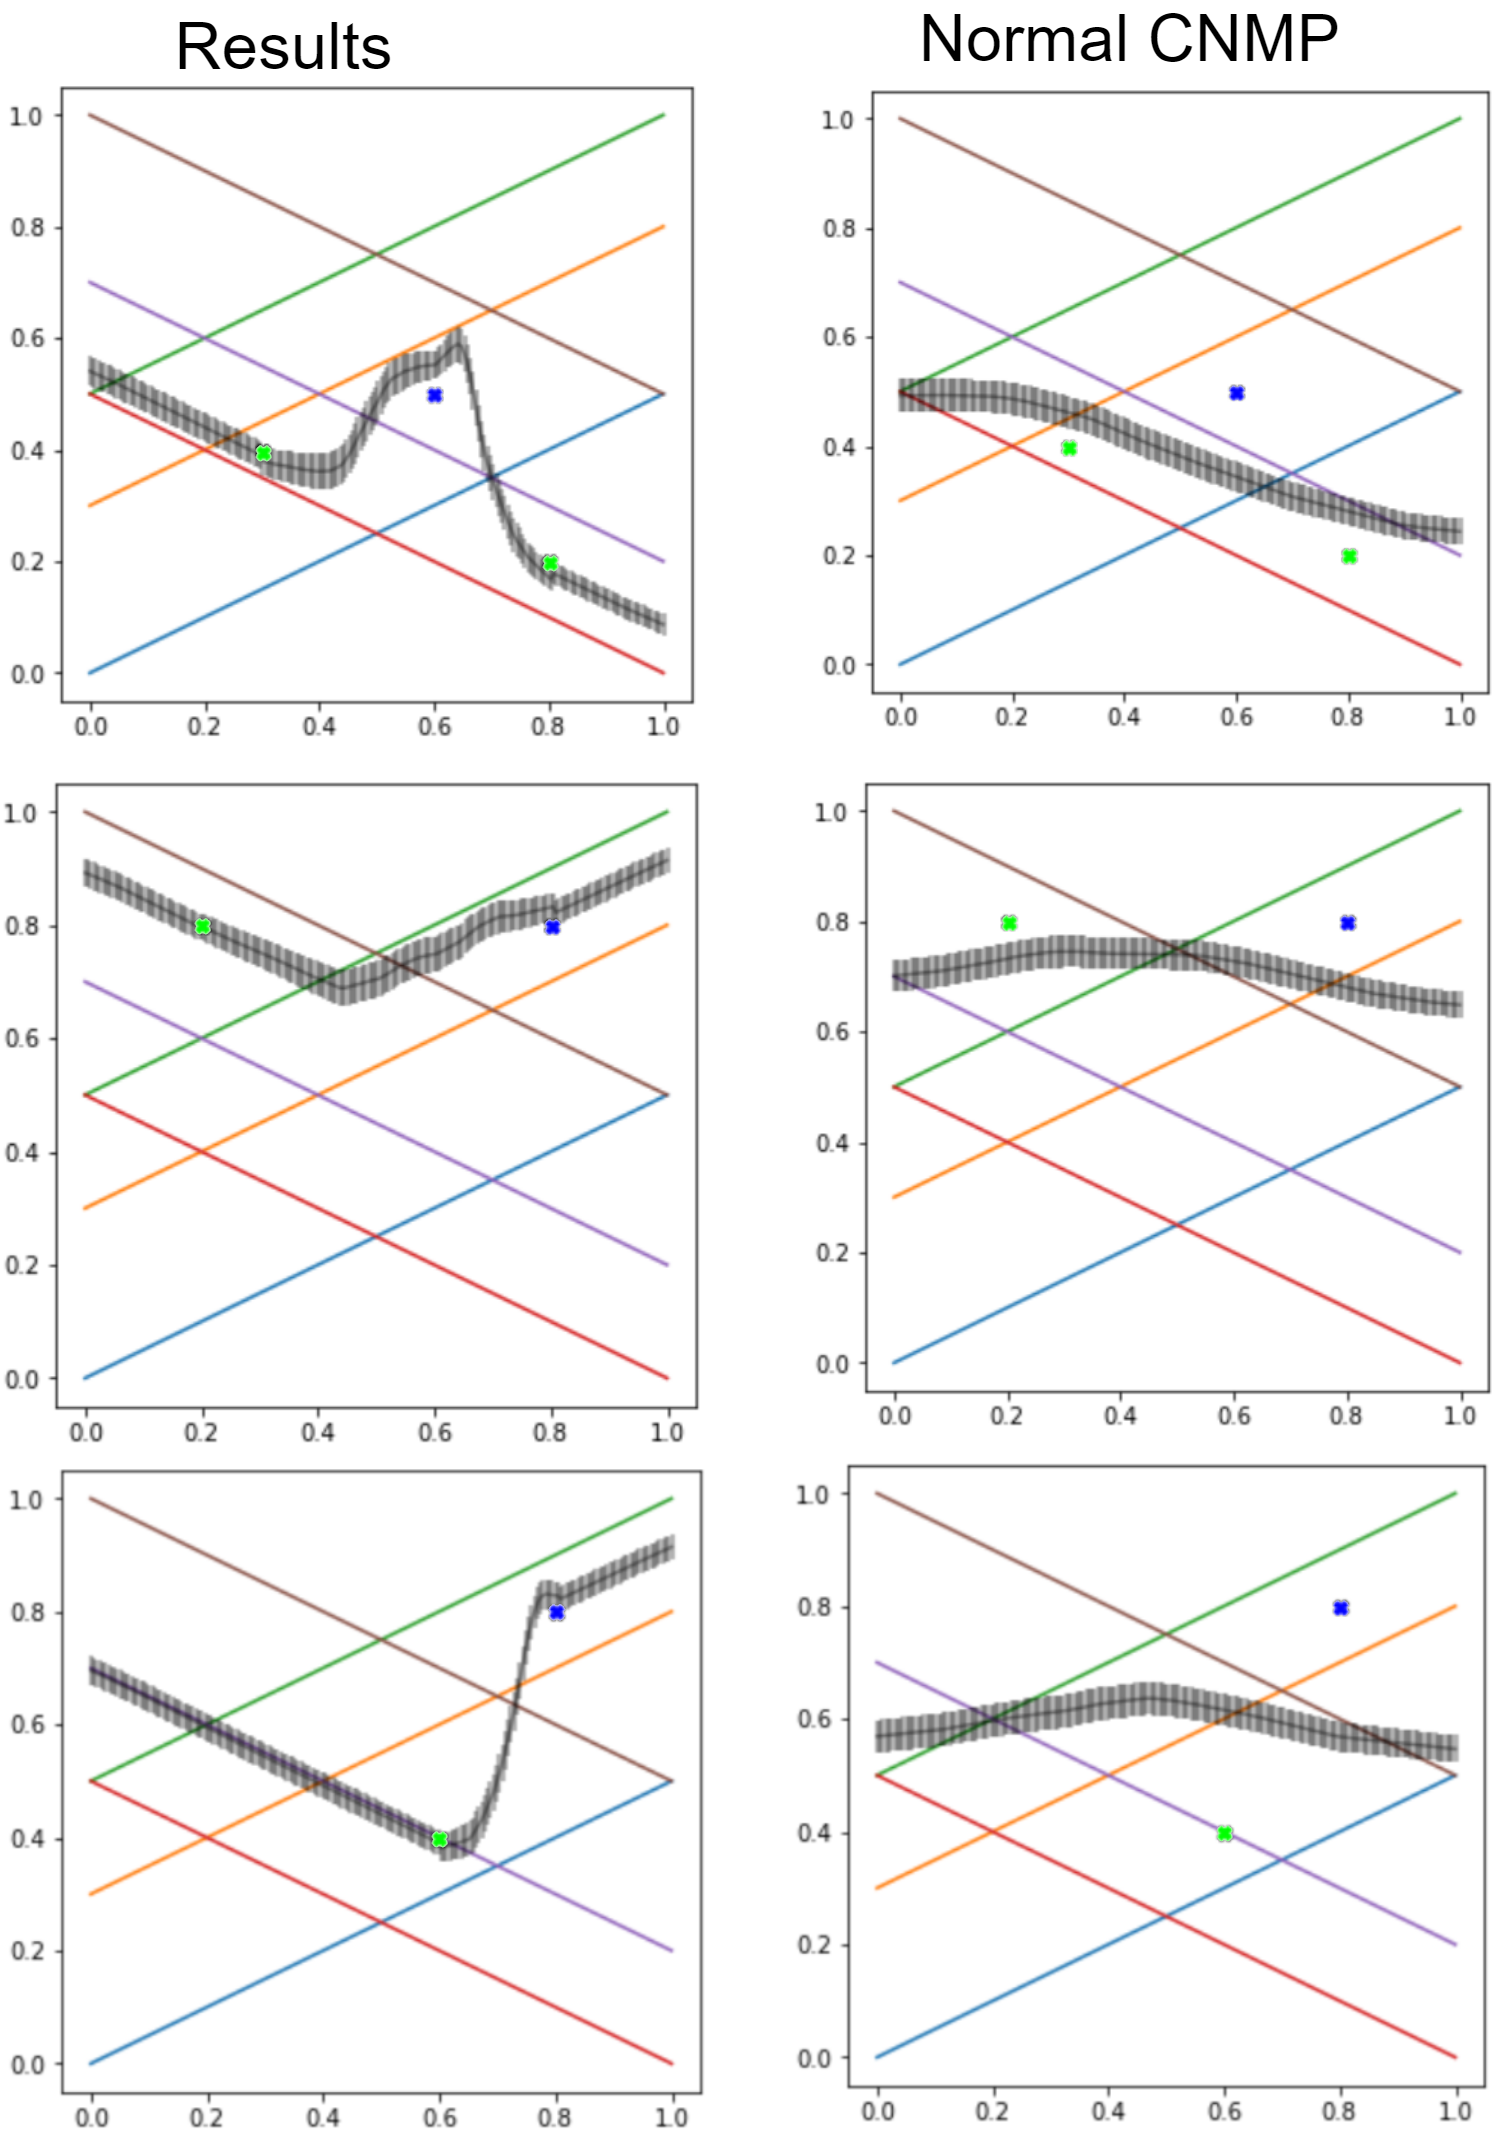
\includegraphics[width=0.9\linewidth]{figures/tp-multiple-shift-results.png}
    \caption{ Final results of multiple tasks transition and comparison with traditional CNMP network. }
    \label{fig:tp-multiple-shift-results}
\end{figure}


\newpage
%%%%%%%%%%%%%%%%%%%%%%%%%%%%%%%%%%%%%%%%%%%%%%%%
\section{End-To-End Skill Concatenation}
%%%%%%%%%%%%%%%%%%%%%%%%%%%%%%%%%%%%%%%%%%%%%%%%
% transition between chapters 
The proposed method in the previous chapter would be really limited if not coupled with the ability to compose the skills in succession. Being able to combine parts is indeed useful, but it will eventually end in the time span of one action, even if we use parts of other ones. To really enhance the potentiality of the network and exponentially enlarge the capacities of the robot, a way to join the skills end-to-end is required. 

% intro
In this part, a method is proposed with which it is possible to concatenate skills one after the other to achieve a goal or reach the final target position or desired state.

% picture of dataset used 
\begin{figure}
    \centering
    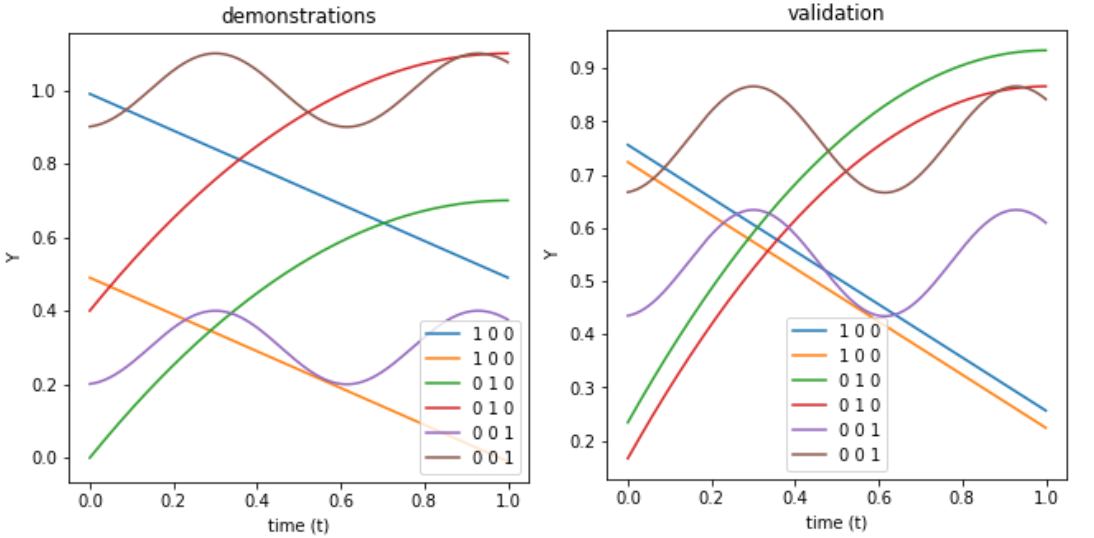
\includegraphics[width=0.9\linewidth]{figures/diff-traj-dataset.png}
    \caption{ Artificial dataset of different skills to concatenate. On the left, there are the demonstrations. On the right, there is the validation. }
    \label{fig:diff-traj-dataset}
\end{figure}

% what required + what subsequently has to be achieved
In order to synthesize a series of actions, the demonstrations have to be initially collected. 
Subsequently, the method presented will combine them end-to-end to reach a desired objective.

% challenge of concatenation without jumps
An immediate challenge presented consists of the concatenation of the movement primitives without incurring in jumps when passing from one to the other. Abrupt jumps in the final movement execution, as previously analyzed, can be dangerous and look unnatural. 

The requirements, also for this research subpart, are indeed that the motions have to be executed with meaning, they have to seem natural, and they have to be safe.  

% challenge different lengths of actions
Another challenge to face is the different lengths of the actions in time and space. Some actions might be faster than others because they are more easily executable, for example, picking an object compared to pouring water. Furthermore, the same actions might last less if performed in different points of space, for example, placing an object in a container next to it or further away. 

% challenge of deciding the right order 
Another possible challenge is choosing the right action sequence to perform. Having all the possibilities from a starting point means that a meaningful choice has to be made. Every action has an effect on the environment, and some of them have a specific order that can not be permutated. Deciding the right order is a complication to solve, 

% simplistic example dataset, but can be extended. What are the demonstrations, what can represent 
For simplicity, the example that will follow will refer to a simple dataset \cref{fig:diff-traj-dataset} that eases the comprehension of the concepts. 
Nevertheless, this method can still be extended to multiple dimensions and more complex scenarios. 

In the dataset artificially generated, two trajectories are provided for each skill. They can resemble any task or movement in time, for example, push or shake an object or move to a position. This dataset enables a clear visualization later on. More realistic but more difficult-to-understand data can be found in the \cref{chap:validation}. 

The different skills, in this case, are given to the same network with the task-parameter option seen in the previous chapter, but it's not necessary. The task parameters are, this time, three, one for each task, and they are boolean, so it's clearly visible which task is queried to the network. The task parameters are visible in the legend of the \cref{fig:diff-traj-dataset}.

% multiple trajectories have to be collected for interpolation
As mentioned in the previous chapter, for every skill, not one but multiple different trajectories are collected. This is not mandatory, as the network can learn with as little as one demonstration. 
However, having multiple expert demonstrations allows the network to generate new unseen ones from interpolation. This extra capability is fundamental since it allows the extension of the effectiveness of the actions from a single point to a whole area or volume. 
Furthermore, having a network that generates new unseen trajectories will allow the method proposed to be validated later for these cases.

The interpolation abilities of the network are validated on the trajectories visible in the right plot. These trajectories enable the code to verify if the movement primitives generated by the network have a minimum error or not. 

% pic of concatenation and jumps 
\begin{figure}
    \centering
    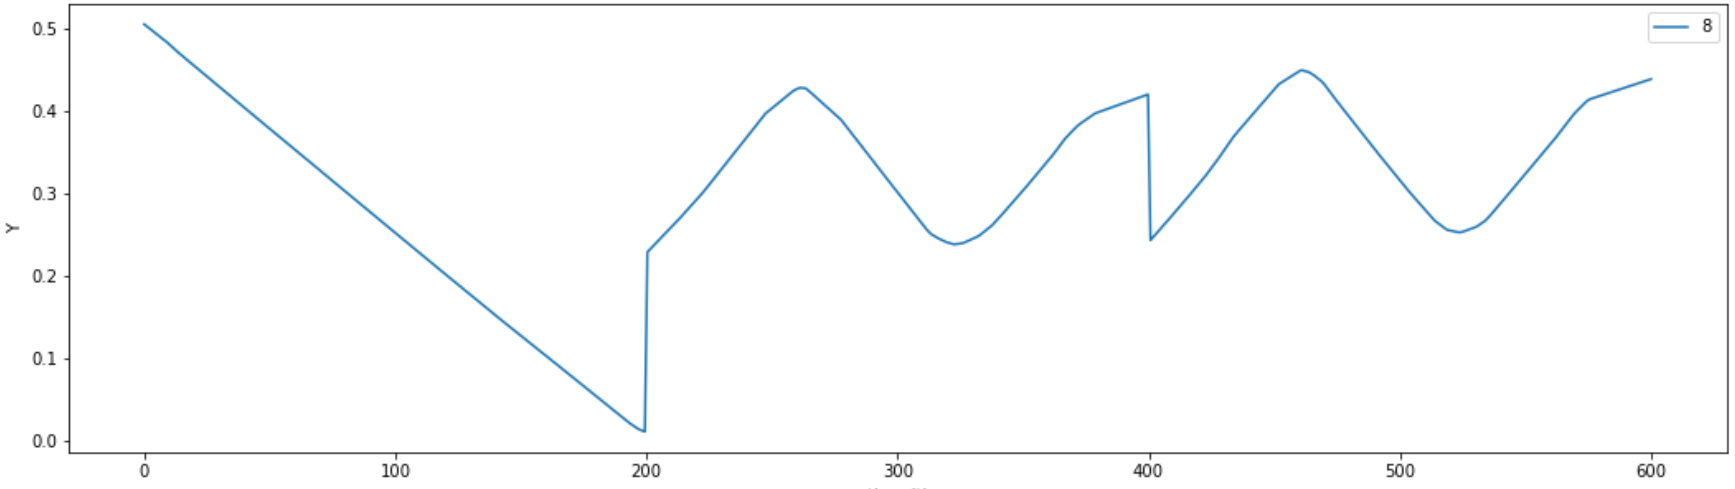
\includegraphics[width=0.9\linewidth]{figures/diff-traj-jump.png}
    \caption{ An example of failing concatenation of skills due to abrupt jumps. }
    \label{fig:diff-traj-jump}
\end{figure}

% concatenation can't be a simple stitch
The joining of multiple trajectories can't be a simple stitch of the previously recorded ones since it will also create abrupt jumps, \cref{fig:diff-traj-jump}. We want to avoid this event for the safety and human-like movements as required but also for a deeper further reason.

Since the network can deal easily with multidimensionality, some dimensions might be added in the future to represent the state of the world. Jumps in the final trajectory must be avoided because the network would allow unmotivated internal world representation changes without being the author of them. However, this is an option that we will explore at the end of this chapter. 

\subsection{CNMP for skill concatenation}
\begin{figure}
    \centering
    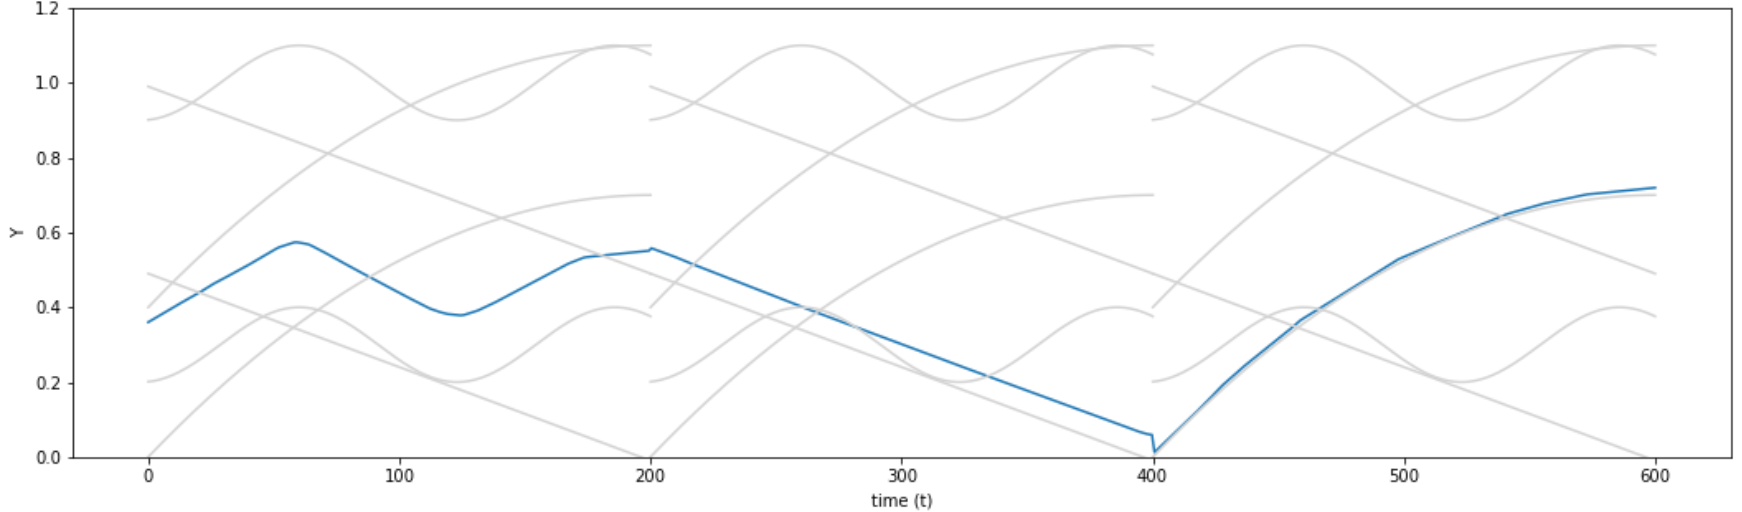
\includegraphics[width=0.9\linewidth]{figures/diff-traj-interpolation.png}
    \caption{ An example of using interpolation with CNMP model to generate new consecutive smooth trajectories. }
    \label{fig:diff-traj-interpolation}
\end{figure}

% CNMP capability interpolation used
To overcome part of the concatenation abrupt changes problem, the ability of CNMP of interpolation is used again. Once the final point of an action is reached, the model is queried to generate the next skills with a conditioning starting point matching it. The model, conditioned on that initial position, will generate the actions required that start from that state, avoiding big discrepancies in the final trajectory generated. 

In \cref{fig:diff-traj-interpolation}, it is possible to see that the first trajectory is the result of the interpolation of the two sinusoidal demonstrations of the dataset depicted in grey. Furthermore, the end of the first trajectory is used as a condition to generate the second one. The second is the interpolation of the two linear functions, also depicted in the background.

It's worth noting that in the example, the output is monodimensional, and the interpolation is simple, but in multidimensional inputs, the CNMPs can interpolate and generate output primitives that are able to interpolate in the whole 3D or joint space. This means that the trajectories of every joint, or 3D axis, won't have abrupt jumps. 

Using a real-life example, if the final position of an action is reached and no other action demonstrated starts from there, the model will use the demonstrated trajectories that start from other points and combine them to generate a skill that starts from that position.

\begin{figure}
    \centering
    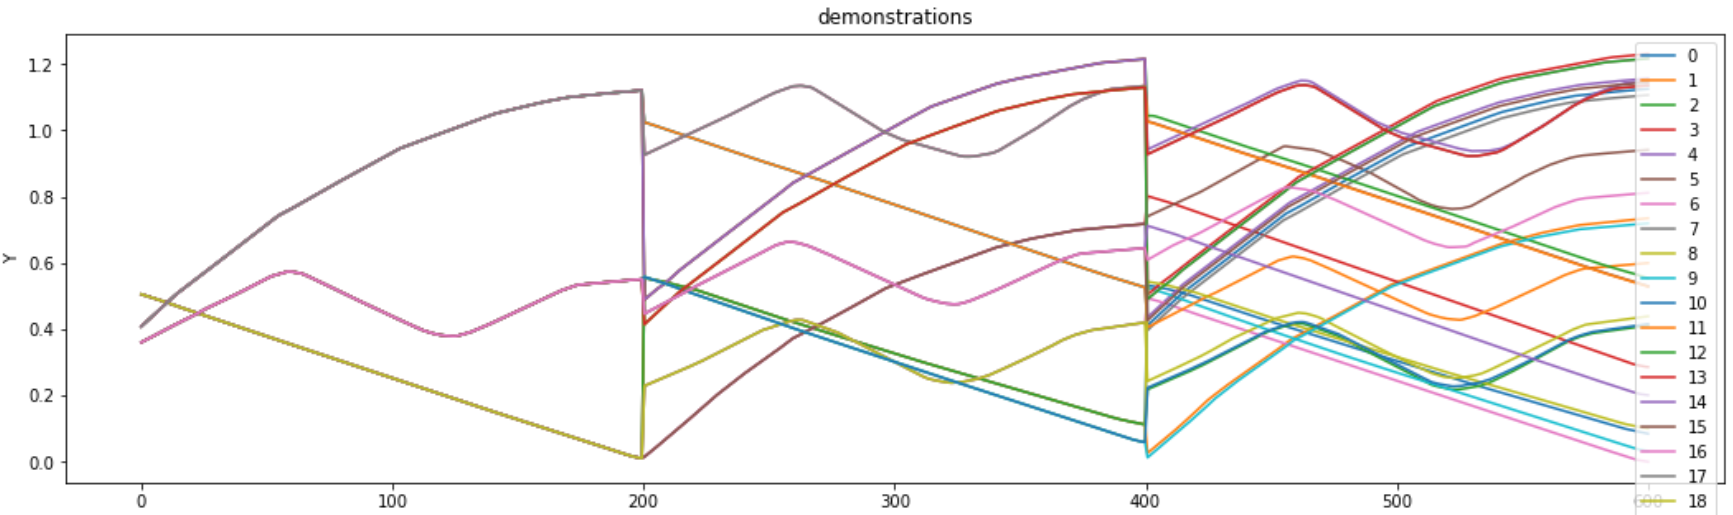
\includegraphics[width=0.9\linewidth]{figures/diff-traj-concat.png}
    \caption{ An example of a recursive concatenation of movement primitives using interpolation abilities of CNMPs. }
    \label{fig:diff-traj-concat}
\end{figure}

% building the graph recursively
At this point, given a starting point, the method proposed recursively builds the graph of all the possible actions, \cref{fig:diff-traj-concat}.
This means that all the actions are evaluated from the starting position, then for all the positions reached, all the actions are generated, and so on. 

The cost of this action is exponential with time; the cost is $O(n_a^{d})$, where $n_a$ is the number of actions available and $n_t$ is the depth number of subsequent actions. The cost is high but can be easily reduced since the network can be queried only for the prediction of the final step, and the queries take milliseconds. 

Furthermore, mechanisms for pruning the tree if a jump is detected can significantly reduce the number of possibilities.
Moreover, the building of the tree can stop once a viable sequence is found to reach the final goal.
Lastly, more informed research is possible with heuristic algorithms that can reduce the steps to find a desired goal.
However, the scope of this research remains to demonstrate the validity of the method, so the optimizations are left for future work.

% extrapolation problem
Even with the interpolation ability, the graph still contains some jumps, and we want to avoid them for the reasons explained previously. This is due to the fact that repeating some actions over and over again will bring the state out of the demonstration range provided to the network. 

The CNMP model shines in the interpolation but lacks the ability to extrapolate from demonstrations. So, if a conditioning point is positioned out of the area between expert demonstrations, the network will simply output the demonstration that is the closest to that point without going further. 

% pic of pruned graph
\begin{figure}
    \centering
    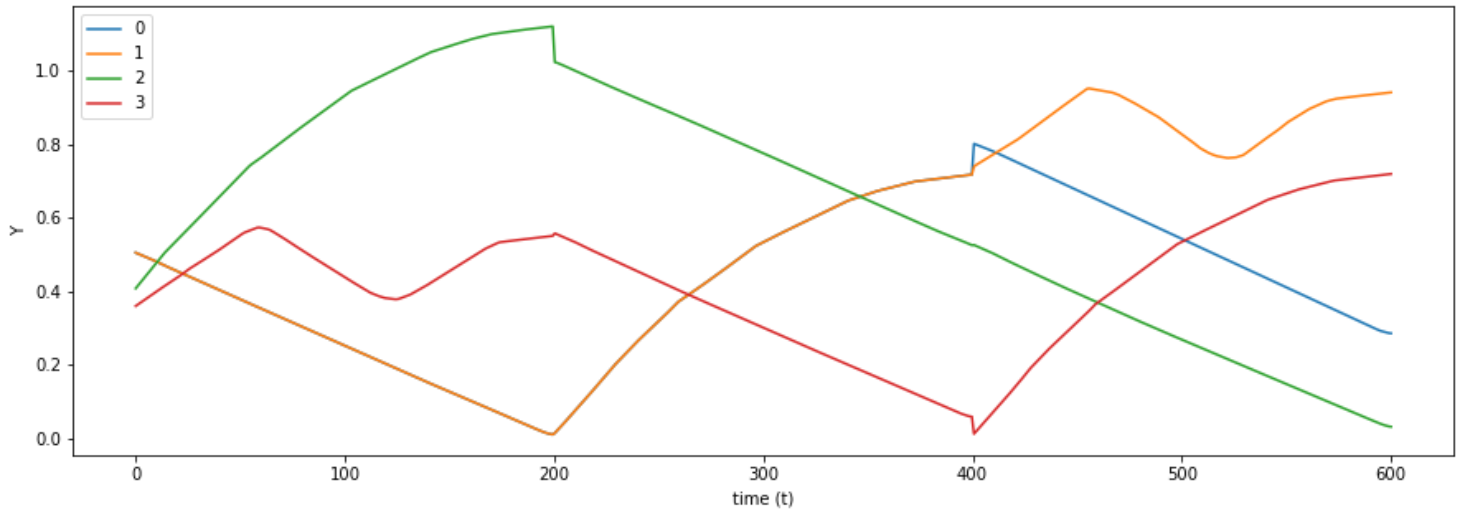
\includegraphics[width=0.9\linewidth]{figures/diff-traj-filtered.png}
    \caption{ An example of filtering the skills generated based on extrapolation limitations. }
    \label{fig:diff-traj-filtered}
\end{figure}

% pruning, using extrapolation as an advantage
This problem actually helps to find the actions that are simply not feasible. For the sake of safety and meaningfulness, it is not actually reasonable to extrapolate the actions demonstrated to the whole space around the agent. For example, concatenating too many push actions might, in real life, exceed the reachability area of the robot or its arm length. 

For this step the assumption taken is that the expert gives demonstrations that are at the limits of the capacity of the robot. This allows the method to derive what is feasible and what is not. 

Consequently, to remove the actions that are not feasible from the option set, it is sufficient to leverage the limitations of the model and just look for big data variations in the sequences generated. After finding them, it's possible to prune the tree from these unfeasible action concatenations.

In \cref{fig:diff-traj-filtered} are presented the selected trajectories generated by the network, with interpolation to avoid jumps, but without extrapolation to avoid the impractical ones. As it is possible to see in the picture, among the four trajectories chosen, it's also present in red the one previously shown in \cref{fig:diff-traj-interpolation} and created using interpolation.

% actions have same length, being small primitives. Future work possible here
All the actions presented in the example have the same temporal length. This is not mandatory but a choice for the sake of simplicity. An extension of this research could include skills that have different durations. Overall, since the majority of movement primitives are simple actions and last a few seconds, this complication was not addressed.  

\subsection{CNMP embedding environment representation}
% trajectories are executable but not always meaningful w/o internal world representation
Trajectories generated in this way are executable and this means that the method works for spatial concatenation. 
On the other hand,  the final goal in this way can be only a position in space or a joint state. 
Although it is really useful to make the robot or the agent reach new places using the previous knowledge, this is limited to the device or, at maximum, the object it can carry.

Upon observation, it's clear that many movement primitives involve an external object or the interaction with the environment around them. Another step in complexity is to develop the method for goals that are not only as a point in time or robot position but also related to the external world. 

The external world introduces a whole new degree of complication because it requires having a degree of knowledge about it. Without this internal representation of the environment, the robot would execute actions that are possible but not meaningful. For example, picking an object that is not present or placing a lid before the pot. 

% will use extra dimensions for world modelling, it's adding a dimension to the output, the opposite of a TP
Since the CNMP model can deal with multidimensional data, the solution proposed is to embed the state changes of the environment in the network. Given a representation of the world, the network can learn how the actions performed change it and the final outcome. The representation can be as simple as a single $x,y$ position of an object manipulated or the whole image of the environment. 

Furthermore, the network's ability to interpolate will make it adaptable to new states, as long as they can be interpolated from demonstrations, and it will be able to predict the outcome of the actions on them. 

\begin{longtable}[c]{|l|l|l|}
\caption{Example of CNMP ability to embed environment representations}
\label{tab:cnmp_env_represenation}\\
\hline
 & left arm & right arm \\ \hline
\endfirsthead
%
\endhead
%
move arm to center & [\textbf{0},1,2] $\rightarrow$ [\textbf{1},1,2] & [0,1,\textbf{2}] $\rightarrow$ [0,1,\textbf{1}] \\ \hline
move arm to its side & [\textbf{1},1,2] $\rightarrow$ [\textbf{0},1,2] & [0,1,\textbf{1}] $\rightarrow$ [0,1,\textbf{2}] \\ \hline
pick and place from side to center & [\textbf{0},\textbf{0},2] $\rightarrow$ [\textbf{1},\textbf{1},2] & [0,\textbf{2},\textbf{2}] $\rightarrow$ [0,\textbf{1},\textbf{1}] \\ \hline
pick and place from center to side & [\textbf{1},\textbf{1},2] $\rightarrow$ [\textbf{0},\textbf{0},2] & [0,\textbf{1},\textbf{1}] $\rightarrow$ [0,\textbf{2},\textbf{2}] \\ \hline
\end{longtable}

A simplistic example is reported. The CNMP model can be trained on both arms of a robot and enable the movement of an object from a position that is reachable only from the left arm to a position that is reachable only to the right arm. 
This action requires the internal knowledge of the position of the object to find the right sequence and not to execute actions that are possible but not meaningful if the object is not in the desired position. 
The object position is encoded with a state $[1,2,3]$ depending on its position from left to right. We assume the left position is only reachable from the left arm, the central position from both arms and the right position from the right arm. 
The arms' positions are encoded in the same way, but by definition, the left arm can reach only the first two and the right arm only the last two. In a real-world scenario, the position of the arm will not be monodimensional but probably multidimensional, but the example is still valid.
The world representation is finally $[PositionLeftArm, PositionObject, PositionRightArm]$. The CNMP model will learn the changes in time of both the arms and the environment representation. The possible demonstrations are depicted in \cref{tab:cnmp_env_represenation}, where pick and place means close the gripper, move to a position, and open the gripper.

Given a condition on the initial state where the object is on the left $[0,0,2]$, the method proposed will build the whole graph of possible actions and resultant environment states. At this point, the sequence for bringing the object from left to right, final state $[0,2,2]$ is:
\begin{enumerate}
  \item $[0,0,2] \rightarrow [1,1,2]$ left arm pick and place from side to center
  \item $[1,1,2] \rightarrow [0,1,2]$ left arm move arm to its side
  \item $[0,1,2] \rightarrow [0,1,1]$ right arm move arm to center
  \item $[0,1,1] \rightarrow [0,2,2]$ right arm pick and place from center to side
\end{enumerate}

It's worth noting that the method doesn't require additional data structures, but it's all embedded in the network. 

This method extension means adding the dimensions normally to the network's input and output. In this way, it's still possible to use the previously presented method to discard the actions that don't bring to a valid state. In the example, it is impossible to move one arm in the center while the other is there so the arms won't collide. 

Moreover, the action possibilities can still be filtered by analyzing abrupt changes in the world representation to understand when an action's output will lead to a state where further actions are not possible. In the example, the object must be in the center to be picked and placed on the side. If not, the generated action will show an abrupt initial change in the environment representation.

% Overall, this doesn't go into planning
While the presented method works out of the box for reaching goals in space, a possible extension for meaningful executions is presented here. Nevertheless, the scope of this work is not action planning, which is a complex topic in robotics beyond the scope of this work.

% shift method is temporally bonded, here adding one action to the set 1) doesn't require adding it in every time slot 2) doesn't require repeating the inital part if it is at the end of the execution 